%%
%% Copyright 2007, 2008, 2009 Elsevier Ltd
%%
%% This file is part of the 'Elsarticle Bundle'.
%% ---------------------------------------------
%%
%% It may be distributed under the conditions of the LaTeX Project Public
%% License, either version 1.2 of this license or (at your option) any
%% later version.  The latest version of this license is in
%%    http://www.latex-project.org/lppl.txt
%% and version 1.2 or later is part of all distributions of LaTeX
%% version 1999/12/01 or later.
%%
%% The list of all files belonging to the 'Elsarticle Bundle' is
%% given in the file `manifest.txt'.
%%

%% Template article for Elsevier's document class `elsarticle'
%% with numbered style bibliographic references
%% SP 2008/03/01
%%
%%
%%
%% $Id: elsarticle-template-num.tex 4 2009-10-24 08:22:58Z rishi $
%%
%%
%%%%%\documentclass[preprint,12pt]{elsarticle}

%% Use the option review to obtain double line spacing
%%  \documentclass[preprint,review,12pt]{elsarticle}

%% Use the options 1p,twocolumn; 3p; 3p,twocolumn; 5p; or 5p,twocolumn
%% for a journal layout:
 \documentclass[final,1p,times]{elsarticle}
%% \documentclass[final,1p,times,twocolumn]{elsarticle}
%% \documentclass[final,3p,times]{elsarticle}
%% \documentclass[final,3p,times,twocolumn]{elsarticle}
%% \documentclass[final,5p,times]{elsarticle}
%%\documentclass[final,5p,times,twocolumn]{elsarticle}%%DOS COLUMNAS


%% The amssymb package provides various useful mathematical symbols
\usepackage{amssymb}
\usepackage{url}
\usepackage{graphicx}
\usepackage{grffile} % get the right dot in filename
\usepackage{epsfig}
\usepackage{algorithm}
\usepackage{algorithmic}
\usepackage{subfigure}
\usepackage{color}
\usepackage{amsmath}
\usepackage{pifont}
\usepackage{multirow}
%% The amsthm package provides extended theorem environments
%% \usepackage{amsthm}

%% The lineno packages adds line numbers. Start line numbering with
%% \begin{linenumbers}, end it with \end{linenumbers}. Or switch it on
%% for the whole article with \linenumbers after \end{frontmatter}.
%% \usepackage{lineno}

%% natbib.sty is loaded by default. However, natbib options can be
%% provided with \biboptions{...} command. Following options are
%% valid:

%%   round  -  round parentheses are used (default)
%%   square -  square brackets are used   [option]
%%   curly  -  curly braces are used      {option}
%%   angle  -  angle brackets are used    <option>
%%   semicolon  -  multiple citations separated by semi-colon
%%   colon  - same as semicolon, an earlier confusion
%%   comma  -  separated by comma
%%   numbers-  selects numerical citations
%%   super  -  numerical citations as superscripts
%%   sort   -  sorts multiple citations according to order in ref. list
%%   sort&compress   -  like sort, but also compresses numerical citations
%%   compress - compresses without sorting
%%
%% \biboptions{comma,round}

% \biboptions{}


\journal{Applied Soft Computing}
\providecommand{\e}[1]{\ensuremath{\times 10^{#1}}}
\begin{document}

\begin{frontmatter}

%% Title, authors and addresses

%% use the tnoteref command within \title for footnotes;
%% use the tnotetext command for the associated footnote;
%% use the fnref command within \author or \address for footnotes;
%% use the fntext command for the associated footnote;
%% use the corref command within \author for corresponding author footnotes;
%% use the cortext command for the associated footnote;
%% use the ead command for the email address,
%% and the form \ead[url] for the home page:
%%
%% \title{Title\tnoteref{label1}}
%% \tnotetext[label1]{}
%% \author{Name\corref{cor1}\fnref{label2}}
%% \ead{email address}
%% \ead[url]{home page}
%% \fntext[label2]{}
%% \cortext[cor1]{}
%% \address{Address\fnref{label3}}
%% \fntext[label3]{}

\title{Studying the effect of population size in distributed evolutionary
  algorithms on heterogeneous clusters}


\author[ugr]{Pablo Garc\'ia-S\'anchez}
\ead{pablogarcia@ugr.es}
\author[ugr]{Gustavo Romero}
\ead{gustavo@ugr.es}
\author[ugr]{Jes\'us Gonz\'alez}
\ead{jesusgonzalez@ugr.es}
\author[ugr]{Antonio Miguel Mora}
\ead{amorag@geneura.ugr.es}
\author[ugr]{Maribel G. Arenas}
\ead{maribel@ugr.es}
\author[ugr]{Pedro A. Castillo}
\ead{pacv@ugr.es}
\author[laseeb]{Carlos Fernandes}
\ead{cfernandes@laseeb.org}
\author[ugr]{Juan Juli\'an Merelo}
\ead{jmerelo@geneura.ugr.es}


\address[ugr]{Department of Computer Architecture and Computer Technology and CITIC-UGR, University of Granada, Granada, Spain. Tel: +34958241778. Fax: +34958248993}
\address[laseeb]{LaSEEB-ISR-IST, Technical University of Lisbon (IST), Lisbon, Portugal}%


\begin{abstract}


Distributed Evolutionary Algorithms are traditionally executed on homogeneous dedicated clusters, 
despite most scientists have access mainly to networks of heterogeneous nodes (for example, desktop PCs in a lab). 
Fitting this kind of algorithms to these environments, so that they
can take advantage of their heterogeneity to save running time, is
still an open problem. The different computational power of the nodes affects
the performance of the algorithm, and tuning or fitting it
to each node properly could reduce execution time. 

Since the distributed Evolutionary Algorithms include a whole range of parameters that influence the performance, 
this paper proposes a study on the population size. This parameter  is one of the most important, 
since it has a direct relationship with the number of iterations needed to find the solution, as it affects
the exploration factor of the algorithm. 
The aim of this paper consists in validating the following hypothesis: fitting the sub-population size to the computational power of the heterogeneous cluster node can lead to an improvement in running time with respect to the use of the same population size in every node. 

Two  parameter size schemes have been tested, an offline and an online parameter setting, and three 
problems with different characteristics and computational demands have
been used. 

Results show
that setting the population size according to the computational power
of each node in the heterogeneous cluster improves the time required
to obtain the optimal solution. 
Meanwhile, the same set of
different size values could not improve the running time  to reach the optimum 
 in a homogeneous
cluster with respect to the same size in all nodes, indicating that the improvement is due to the interaction of the different hardware
resources with the algorithm. In addition, a study on the influence of
the different population sizes on each stage of the algorithm is
presented. This opens a new research line on the fitting (offline
or online) of parameters of the distributed Evolutionary Algorithms to the computational power of the devices.





 
\end{abstract}

\begin{keyword}

Evolutionary Algorithms \sep Genetic Algorithms \sep Distributed computing \sep Parameter Tuning \sep Parameter Control

\end{keyword}

\end{frontmatter}

\section{Introduction}
\label{sec:intro}



Evolutionary Algorithms (EAs) are a general method for solving
optimization and search problems inspired by the evolution of species
and its underlying mechanism, natural selection. These algorithms work
on a population of encoded
possible solutions, called {\em individuals}, every one competing with others according to their
{\em fitness} (quality or cost of the solution they encode). The population evolves, with iterations of the algorithm (or {\em generations}), 
by means of selection and recombination/mutation operators, 
creating a new set of candidates. This goes on until a {\em stopping criterion}
(e.g. number of generations) is met. The fitness function, which describes the target problem,  expresses
the quality of the solution, giving the grade of adaptation of an
individual.

The performance of an EA can be measured by the running time required to find the optimal value 
and/or by the quality of the solution attained in a fixed time. The performance is affected by a set 
of parameters, such as the crossover rate, or population size, among others. 
Population size has been studied as a fixed \cite{SizingHarik99} or adaptive 
\cite{SelfRegulatedSizeFernandes06,AdaptiveLobo07} value, as it has a significant impact on the efficiency of an EA \cite{ShrinkageLaredo09}.

Performance can also be improved using Distributed EAs (dEAs) \cite{MULTIKULTI}, where the algorithm is run on a set of nodes simultaneously,
working with different sub-populations (or islands) at the same
time. One or more individuals are
interchanged (migrated) periodically between sub-populations, which are connected
following a specific topology. Figure \ref{fig:islands} shows the island
model with a ring topology. 


\begin{figure}[htb]
\centering
\epsfig{file=ring.eps, width = 7cm}
\caption{Island model scheme using a neighborhood ring topology.}
\label{fig:islands}
\end{figure}






Cant{\'u}-Paz, in \cite{CantuPazTopologies99}, published a theoretical study about population size, migration rate and the degree of the topology.  This kind of algorithms has been usually executed on homogeneous clusters \cite{MULTIKULTI,Wakunda97EVA}, being used with the same
parameters in all nodes (homogeneous dEAs), or with different
parameters (heterogeneous dEAs) \cite{garcia2014randomized,tanabe2013evaluation,HETEROGENEOUSPARAMETERS}. 



As previously said, population size is a key factor for the performance 
of dEAs \cite{ShrinkageLaredo09}, so this paper investigates whether
adapting the sub-population size of each node in a distributed
Evolutionary Algorithm can leverage the
computational capabilities of a heterogeneous cluster.                             

This is motivated by new trends in distributed computing, such as Cloud Computing \cite{Derby13Cloud}, GRID
\cite{OPENSCIENCEGRID} or Service Oriented Science \cite{GLOBUS}, which are
leading to heterogeneous computational devices, such as laptops,
virtual machine instances, 
GPUs \cite{Acosta13GPUs},
tablets or desktop PCs, working in the same
environment. Thus, many laboratories, which do not include classic
clusters but the usual desktop and laptop computers, should be able to leverage
this motley set as a heterogeneous cluster. 

It  has  been shown that
\cite{HETEROGENEOUSHARD} asynchronous dEAs with the same parameter
configuration are even 
more efficient in time and the number of evaluations in reaching the optimal solution on this kind of environments  than on clusters with
homogeneous devices. This can be explained by different reasons, such
as different memory access times, cache sizes, 
or even implementation
languages or compilers in each machine, leading to a different
exploitation/exploration rate of the search space \cite{HETEROGENEOUSHARD}. 


These facts have motivated the study of a combination of both ideas in
this paper: asynchronous dEAs on a heterogeneous set of nodes with different
parameter values fitted to each node. The concept {\em parameter fitting} is proposed in this work to distinguish with respect the term {\em parameter adaptation} defined by Eiben in \cite{Eiben05Shared}. Our concept specifies that the parameter values are set (online or offline) taking into account the computational power of the nodes, while the parameter adaptation implies a modification (online) of the parameters taking into account the information provided by the algorithm itself (for example, a variation in the average fitness value).

In this case, the parameter to
be fitted to the computational power of each node has been the
sub-population size of each island. 
The population size is of capital importance in the accuracy and
convergence speed of an EA. The population is a repository of the
building-blocks that an evolutionary computational process recombines
and mutates in order to improve the average fitness of the population
and, eventually, find the optimal solution to the target-problem. If
the supply of building-blocks is insufficient, selection and genetic
drift will probably guide the search towards premature convergence to a
local optimum (or the EA becomes too dependent on the randomness of
the mutation operator). Larger populations guarantee a more diverse
supply of building-blocks (higher genetic diversity) and are more
likely to overcome premature convergence. However, in large
populations, convergence speed is the payoff for accuracy: in general,
when the population size of an EA grows, the convergence speed is
reduced \cite{Cantu02Multiple}. When having different processors with different computational
power computing sub-populations of an EA, it may be a good policy to
distribute the individuals in a way that less efficient nodes are
assigned with smaller populations, having smaller diversity. 
This solution not only integrates
within an EA two different types of evolutionary search (fast, with
the smaller populations, and accurate, with the larger), but also puts
on the most efficient nodes the burden of computing larger
sub-populations. This combination can reduce computation time
as slower nodes can exploit solutions without premature convergence and,
 at the same time, benefit from the diversity of the faster ones. 

In this work, a heterogeneous distributed system has been used to
answer  the following research questions:
\begin{itemize}
 \item Can an asynchronous distributed EA be fitted to leverage the capability of a
   heterogeneous cluster? 
 \item How does the fitting of the sub-population size to the computational power affect the running time and number of evaluations?
 \item Is there any difference between using the same sub-population sizes on a homogeneous and a heterogeneous cluster?
 \item How is each stage of the algorithm (selection, recombination, mutation, replacement and migration) affected by the different
   configurations?
\end{itemize}



The rest of the work is structured as follows: after a background in the algorithm parameter fitting to computational substrate in dEAs, 
 the developed algorithms and experimental setting (Section \ref{sec:experiments}) are presented. 
Then, the results of the experiments are shown (Section \ref{sec:results}), followed by conclusions and suggestions for future work lines.


%%%%%%%%%%%%%%%%%%%%%%%%%%%%%%  SOA  %%%%%%%%%%%%%%%%%%%%%%%%%%%%%%
%
\section{Background on tuning and fitting EAs on heterogeneous clusters}
\label{sec:soa}

Fitting algorithm parameters to available heterogeneous computational resources
usually leads to improved performance
\cite{AutomaticallyConfiguringStyles12}. An easy way to take advantage
of the available resources is  balancing the load
\cite{PARALLELIMPLEMENTATION,Martinez11Nondedicated} so that workloads are distributed across multiple
elements. However, assigning equal tasks  to each node in
heterogeneous clusters may result in suboptimal performance
\cite{LoadBalancingBohn02}. 



One of the problems in parameter tuning and adaptation on heterogeneous clusters is 
the computational load representation. It depends on the algorithm, size of the problem, 
language, compiler or hardware characteristics, so the results obtained from artificial 
benchmarks, such as  Linpack \cite{LinpackEndo10}, should not be extolled as identificative 
of the system performance \cite{LinpackDongarra03}. For example, in the work of Garamendi 
et al. \cite{PARALLELIMPLEMENTATION},  a small benchmark was executed on all nodes at the beginning
of the algorithm in order to distribute individuals of an Evolutionary Strategy
 (ES), following a master-slave model. The computational load by artificial benchmarks may not  
 represent the correct load of the algorithm accurately, so, as proposed in this paper, information 
 about the algorithm itself should be used for calibration.

 Besides, dEAs are not usually based in the master-slave paradigm for
load balancing (unlike the Global Parallel EAs
\cite{alba2002parallelism}), so setting different sub-population sizes
may affect the algorithmic performance if used on heterogeneous
environments. 

In other works, there is no direct relation between the algorithm parameters and the
computational resources of the nodes. For example, Dom\'inguez et al. \cite{HYDROCM} 
divided the available devices in ``faster'' and ``slower'' nodes to create a distributed hybrid 
meta-heuristic that combines two different methods: Genetic Algorithms (GAs) and Simulated
Annealing (SA). Their system executes the GAs, heavier in computational
terms, in the faster nodes, and
simpler meta-heuristics (SA) in the slower ones, obtaining better results
than other configurations.  Gong et al. in \cite{HETEROGENEOUSTOPOLOGY} also ordered 
the nodes by their computational power to test different topology configurations in a distributed EA.
Besides from ordering the nodes taking into account 
only their previously known computational resources, the results of previous works were not compared in a homogeneous 
cluster to validate if the fitting takes advantage of the heterogeneity 
of the cluster, as proposed in this paper.

The heterogeneous computational performance of nodes or network speed can affect the performance of an algorithm. In \cite{HETEROGENEOUSHARD},
 Alba et al. compared a dGA, 
 on homogeneous and heterogeneous clusters. 
 Super-linear performance in terms of number of iterations to find the optimum was obtained on the heterogeneous ones,
 being more efficient than the same algorithm running on homogeneous
 machines. However, the parameter setting was the same in both
 clusters and the authors did not fit the parameters to the machines used. 



Fitting algorithm parameters to computational nodes derives on heterogeneous parameter sets. These sets can improve the results on homogeneous hardware, for example, setting a random set of parameters in each homogeneous node can also increase the
performance of a dGA, as explained by Gong
and Fukunaga in \cite{HETEROGENEOUSPARAMETERS}. That model
outperformed a tuned canonical dGA with the same parameter values in
all islands. Other approaches \cite{PanaceasClune05,ParallelGATongchim02} optimise sets of heterogeneous parameters using meta-GAs. Single parameter fitting has also been  studied. For example, adapting the migration rate produced better
results than homogeneous periods, as explained by Salto and Alba in
\cite{HETEROGENEOUSMIGRATION}. This indicates that heterogeneous parameters
 may lead to an increase of performance, so it is necessary to validate if the 
 performance is due to the parameter set or by the heterogeneous devices combination.



This work is focused on the sub-population sizes, as this parameter has been previously studied in different works due to its huge impact on the results. In the work of Weber et al. \cite{DifferentialWeber09} two different sub-population sizes are used: higher size value for exploration, and a variable lower size value for exploitation. Schlierkamp-Voosen et al. \cite{AdaptationSizesSchlierkamp96} proposed a quality measure to be used in each sub-population to adapt the size, also taking into account the migration and crossover mechanisms. However, these works are based on the competition of sub-populations, taking into account only the information provided by the fitness of the population, and not by the machines that are executing the distributed EAs.


In this work, the sizes of the sub-populations of a dEA are fitted (offline and online) to the computational power of each machine, using the information obtained from the algorithm itself, and compared on different hardware systems.
 To the best of our knowledge, there are no works that
 modify parameters of the EA, such as the size, depending on the
 node where the island is being executed, while taking into account information provided by the execution of the algorithm. 


 


%%%%%%%%%%%%%%%%%%  Experiments  %%%%%%%%%%%%%%%%%%%
\section{Experimental setup}
\label{sec:experiments}
In this section two different parameter setting schemes are proposed to test if fitting the sub-population sizes of an asynchronous dEA to the nodes of a  heterogeneous cluster leads to time reduction. In the field of  Evolutionary Computation (EC) there are two different approaches about the algorithm parameter setting: {\em parameter tuning} and {\em parameter control} \cite{PARAMETERTUNING}. The former consists in establishing a good set of parameters before the run (offline), that do not change  during the execution. Parameter control refers to setting up a number of  the EA parameters  and changing these values in running time (online). 

In this study, a dEA with the same sub-population sizes  has been executed in the heterogeneous cluster until the optimal solution is found, as a baseline. Then, the obtained number of generations has been used, to  distribute the number of individuals proportionally among the nodes, that is, offline. The same set of sizes is used in a homogeneous cluster (as control system) to validate if the changes in performance are due to the parameters or the fitting to the nodes. Finally, an online parameter setting that extracts relative information about the performance of the nodes has been tested to validate our approach. 

%MARIALUISA: Pablo cambia has been used, to proportionally distribute the number of individuals por to distribute the number of individuals proportionally; cambia an homogeneous por A homogeneous; cambia extract por EXTRACTS”



\subsection{Algorithm used}
The experimentation is focused on a distributed GA, one of the most extended EAs \cite{GeneticAlgorithmsEiben03}. Algorithm \ref{alg:EA} shows the pseudo-code of the  used algorithm.
It is a steady-state approach, i.e. in every generation the offspring is mixed with the parents and the worst individuals are removed. Also, each pair of parents selected during crossover generates two new individuals for offspring. That is, in each generation, a crossover with a rate of 0.5 selects half of population for crossover and generates an equal number of offspring. The selected neighbourhood topology for migration between islands (nodes) is a ring (see Figure \ref{fig:islands}). The best individual is sent to the neighbour in the ring, after a fixed number of generations in each island. The algorithm stops when the optimum (the solution to the problem) is found.  



\begin{algorithm}[htb]

\begin{algorithmic}
\STATE population $\gets$ initialisePopulation()
\WHILE {stopping criterion not met}
    \STATE parents $\gets$ selection(population)
    \STATE offspring $\gets$ recombination(parents)
    \STATE offspring $\gets$ mutation(offspring)
    \STATE O $\gets$ offspring.size {\em //O is also equal to the number of parents selected}
    \STATE population $\gets$ population + offspring
    
    \IF {time to migrate}
      \STATE migrants $\gets$ selectMigrants(population)
      \STATE remoteBuffer.send(migrants)
    \ENDIF

    \IF {localBuffer.size $\neq$ zero}
      \STATE immigrants $\gets$ localBuffer.read()
      \STATE I $\gets$ immigrants.size()
      \STATE population $\gets$ population + immigrants
    \ENDIF
    
    \IF {localBuffer.size $\neq$ zero}
      \STATE population $\gets$ population + localBuffer.read()
    \ENDIF
    \STATE population $\gets$ population - population.getTheWorst(O + I)
\ENDWHILE

\end{algorithmic}

\caption{Pseudo-code of the used dEA: a distributed Genetic Algorithm (dGA).}
\label{alg:EA}
\end{algorithm}




\subsection{Problems}


Although results may be independent of the problem, as an adaptive algorithm cannot replace a specific problem adaptation \cite{PanaceasClune05}, different types of problems that cover different characteristics
and computational demands have been used in this work.

In these experiments, the Massively Multimodal Deceptive
Problem (MMDP) \cite{goldberg92massive},  the OneMax problem
\cite{ONEMAX}, and the Rosenbrock Function \cite{CEC2005_Benchmark} have been used. Each one requires different actions/abilities by the GA
at the level of population sizing, individual selection and
building-blocks mixing. Also, these problems have been used previously in other parameter adaptation algorithms, such as \cite{ParallelGATongchim02} (MMDP and OneMax) and \cite{DifferentialWeber09,AdaptationSizesSchlierkamp96} (Rosenbrock). 



The MMDP
 is designed to be difficult for an EA, due to
its multimodality and deceptiveness. Deceptive problems are functions where low-order building-blocks do not combine to form higher order building-blocks. Instead, low-order building-blocks may mislead the search towards local optima, thus challenging search mechanisms. MMDP is composed of $k$ sub-problems of 6 bits each one ($s_i$). Depending on
the number of ones (unitation) $s_i$ takes the values shown in Table \ref{table:mmdpvalues}.  

\begin{table}

\centering
{\footnotesize 
\caption{ Basic deceptive bipolar function ($s_i$) for MMDP.}
\label{table:mmdpvalues}
\begin{tabular}{|c|c|}
\hline
{\em Unitation} & {\em Sub-function value}\\
\hline \hline
0 & 1.000000 \\
\hline
1 & 0.000000 \\
\hline
2 & 0.360384 \\
\hline
3 & 0.640576\\
\hline
4 & 0.360384\\
\hline
5 & 0.000000\\
\hline
6 & 1.000000\\
\hline

\end{tabular}
}


\end{table}


The fitness value is defined as the sum of the $s_i$ sub-problems with an optimum of $k$ (Equation \ref{eq:mmdp}).
The search space is composed of $2^{6k}$ combinations from which there
are only $2^k$ global solutions with $2^k$ deceptive
attractors. Hence, a search method has to find a global solution
out of $2^{5k}$ additionally to deceptiveness. In this work, three different problem sizes have been used: $k=25$ (150 bits), $k=40$ (240 bits) and $k=50$ (300 bits). 

\begin{equation}\label{eq:mmdp}
f_{MMDP}(\vec s)= \sum_{i=1}^{k} fitness_{s_i}
\end{equation}


OneMax is a simple linear problem that consists in maximising the number of ones in a binary string. That is, maximise the expression specified in Equation \ref{eq:onemax}.
\begin{equation}\label{eq:onemax}
f_{OneMax}(\vec{x}) = \sum_{i=1}^{N}{x_{i}}
\end{equation}

In this case, three different string sizes have been used: 5000, 10000 and 15000.
%%%%%%%%%%%%%%%%%%

Finally, the Shifted Rosenbrock function is defined in Equation \ref{eq:rosenbrock}.


\begin{equation}\label{eq:rosenbrock}
%f_{Rosenbrock}(\vec{x})= \sum_{i=1}^{D-1} (100 \cdot (z_{i}^{2}-z_{i+1}^{2}) +                                      (z_{i}-1)^2)+f_{bias}
f_{Rosenbrock}(\vec{x}) = \sum^{D-1}_{i = 1} [100(z_{i + 1} - z^2_i)^2 + (z_i - 1)^2] + f_{bias}
\end{equation}

With $z=x-o+1$ and $\vec{x}=[x_1,x_2,...,x_D]$, and considering $D$ as the number of dimensions, and $o=[o_1,o_2,...,o_D]$ as the shifted global optimum.

This is a multi-modal shifted function, which is non-separable and scalable and it presents a very narrow valley from local optimum to global optimum. It is part of the CEC 2005 Benchmark \cite{CEC2005_Benchmark}, and the optimum is set to the value 390 (with an error of 0.001). Three different chromosome lengths have been used: 10, 30 and 50.

%%%%%%%%%%%%%%%%%


\subsection{Hardware and parameter configurations}




The main objective of this work is testing parameter fitting to hardware. Thus, different configurations should be used to compare and validate if the change in the parameters depends on the parameters, the hardware heterogeneity, or a combination of both. Therefore, the same parameters are used in a homogeneous cluster as a control system for the experiments.
Five configurations of hardware and parameter settings were tested:


\begin{itemize}
\item HoSi/HeHW: Homogeneous Size/Heterogeneous Hardware. The same sub-population size in each island on a heterogeneous cluster.
\item HeSi/HeHW: Heterogeneous Size/Heterogeneous Hardware. Different sub-population sizes in each island on a heterogeneous cluster.
\item HoSi/HoHW: Homogeneous Size/Homogeneous Hardware. The same sub-population size in each island on a homogeneous cluster.
\item HeSi/HoHW: Heterogeneous Size/Homogeneous Hardware. Different sub-population sizes (the obtained for HeSi/HeHW) in each island on a homogeneous cluster.

\item AdSi/HeHW: Adaptive Size/Heterogeneous Hardware. Online fitting of sub-population sizes in each island on a heterogeneous cluster.
\end{itemize}

Two different computational systems were used: a {\em heterogeneous cluster} and a {\em homogeneous cluster}. The first one is formed by different computers of our lab with different processors, operating systems and memory size. The latter is a dedicated scientific cluster formed by homogeneous nodes. Table \ref{tabcomputers} shows the features of every system and the name of the nodes.

\begin{table*}
\centering{\footnotesize 
\caption{Details of the clusters used: a homogeneous cluster (Ho), and a heterogeneous cluster (He)}
\begin{tabular}{|c|c|c|c|c|c|} \hline
{\em Name}     & {\em Processor}  & {\em Memory}  & {\em Operating System}  & {\em Network} & {\em Storage}  \\ \hline
\multicolumn{6}{|c|}{Homogeneous cluster} \\ \hline
HoN[1-8] &  Intel(R) Xeon(R) E5320 ($4\times1.86$GHz) & 4GB & CentOS 6.7           & 1GbE   & Local \\ \hline
\hline
\multicolumn{6}{|c|}{Heterogeneous cluster} \\ \hline
HeN1  &  AMD A10-7700K APU  ($4\times3.4$GHz)         & 7GB   & Fedora 21    (64b) & 1GbE   & Local \\ \hline
HeN2  &  Intel(R) Core(TM)2 Q6600 ($4\times2.4$GHz)   & 4GB   & Ubuntu 12.04 (64b) & 1GbE   & Local \\ \hline
HeN3  &  AMD Phenom(tm) 9950 ($4\times1.3$Ghz)        & 4GB   & Ubuntu 13.10 (32b) & 100MbE & Local \\ \hline
HeN4  &  Intel(R) Pentium(R) D ($2\times2.4$GHz)      & 2GB   & Fedora 19    (64b) & 1GbE   & NAS   \\ \hline
HeN5  &  Intel(R) Core(TM) i5-4430 ($4\times3.00$GHz) & 16GB  & Ubuntu 14.04 (64b) & 1GbE   & Local \\ \hline
HeN6  &  Intel(R) Core(TM)2 Q6600 ($4\times2.40$GHz ) & 8GB   & Ubuntu 11.10 (64b) & 100MbE & Local \\ \hline
HeN7  &  Intel(R) Core(TM) i7 870  ($4\times2.93$GHz) & 8GB   & Fedora 17    (64b) & 1GbE   & Local \\ \hline
HeN8  &  Intel(R) Core(TM)2 Q8200 ($4\times2.33$GHz) & 4GB   & Ubuntu 14.04 (64b) & 1GbE   & Local \\ \hline
\end{tabular}
\label{tabcomputers}
}
\end{table*}

To study the scalability, two different numbers of nodes were used in each problem and configuration: 4 nodes (from HeN1/HoN1 to HeN4/HoN4, referred as  {\em 4X} configuration for the rest of the paper) and 8 nodes (from HeN1/HoN1 to HeN8/HoN8, referred as {\em 8X} configuration). The same amount of nodes has been  used previously in other works on dEAs on heterogeneous environments \cite{HETEROGENEOUSHARD,HYDROCM,Salto13Distributed}.

The global population size was set to 1024 individuals. Other researchers who investigate in dEAs on heterogeneous environments have used 512 individuals (see the works \cite{HYDROCM,Dominguez13HydroCM,Salto13Distributed}). However, as using 512 individuals in  preliminary runs obtained extremely low sub-population sizes, a larger value was used. A population of 1024 is large enough to test different sub-population sizes in different number of computational nodes (4 and 8), allowing a better distribution among them. The stopping criterion for all approaches used in this work is to find the optimum of the problem, so that all runs have always finished when the optimum has been found in one of the nodes. This stopping criterion has been considered as Alba et al. did in \cite{EVALUATIONPARALLEL}, since it offers a fair way to compare the running time and behaviour of the tested configurations. Two-point crossover was used, as it has been used previously in studies on parallel GAs  for binary problems \cite{CantuPazTopologies99}, and BLX-0.5 for real coded dEAs \cite{Robles09ParallelFuzzy}.

\subsubsection{Homogeneous Size configuration}



In this configuration, each node has the same number of individuals, so the total amount is 1024.  The algorithm was run 40 times per problem instance on the homogeneous (HoHW) and heterogeneous clusters (HeHW).  The average number of generations in each node of the HeHW cluster is shown in Table \ref{table:generations4X} (for 4X) and Table \ref{table:generations8X} (for 8X). Note how the generations attained and their proportion in every node to reach the optimum depend on the problem considered, besides the hardware.

\begin{table*}
\centering{
\caption{Average number of generations (and proportion) in each node of the 4X HoSi/HeHW configuration when the optimum is found in 40 runs. These values were used to set  the sub-population sizes proportionally in 4X HeSi (the offline approach).}

\begin{tabular}{|c|c|c|c|c|c|} \hline
{\em Instance} &         & {\em HeN1}     & {\em HeN2 }     & {\em HeN3 }    & {\em HeN4 }  \\ \hline
\multicolumn{6}{|c|}{{\em MMDP problem}} \\ \hline
\multirow{3}{*}{150} & Generations   & 25438  & 17515  &  14030  & 642 \\ \cline{2-6}
                     & Proportion (\%)   & 44.14  & 30.39  & 24.34   &  1.11   \\ \cline{2-6}
                     & Sub-pop. size & 452    & 311    & 249     &  12       \\ \hline
\multirow{3}{*}{240} & Generations   & 214425 & 159545 & 122233  & 6899  \\ \cline{2-6}
                     & Proportion    & 42.62  &  31.71 &  24.30  & 1.37       \\ \cline{2-6}
                     & Sub-pop. size & 436    &  324   & 248     & 14      \\ \hline
\multirow{3}{*}{300} & Generations   & 380205 & 276780 & 203157  & 7730     \\ \cline{2-6}
                     & Proportion  (\%)  & 43.81  & 31.89  & 23.41   & 0.89    \\ \cline{2-6}
                     & Sub-pop. size & 448    &  326   & 240     & 10    \\ \hline                     
\multicolumn{6}{|c|}{{\em OneMax problem}} \\ \hline
\multirow{3}{*}{5000} & Generations   & 2486  &  1575  & 1377    & 512      \\ \cline{2-6}
                     & Proportion  (\%)  &  41.78 &  26.47 &  23.14  & 8.61   \\ \cline{2-6}
                     & Sub-pop. size &  428   &   272  & 236     & 88    \\ \hline    
\multirow{3}{*}{10000} & Generations   & 5135 & 2862   & 2658    & 1125      \\ \cline{2-6}
                     & Proportion  (\%)  &  43.59 &  24.30 &  22.56  & 9.55     \\ \cline{2-6}
                     & Sub-pop. size &  446   & 248    &  232    & 98   \\ \hline    
\multirow{3}{*}{15000} & Generations & 7922   & 4068   & 4092    & 1653      \\ \cline{2-6}
                     & Proportion  (\%)  &  44.67 &  22.94 &  23.07  & 9.32     \\ \cline{2-6}
                     & Sub-pop. size & 457    & 235    & 236 & 96      \\ \hline    
\multicolumn{6}{|c|}{{\em Rosenbrock function}} \\ \hline
\multirow{3}{*}{10} & Generations   & 74736   &47019   & 52293   & 601     \\ \cline{2-6}
                     & Proportion (\%)   & 42.79  &  26.92 &   29.94 &   0.34    \\ \cline{2-6}
                     & Sub-pop. size &  441  & 270     & 309     & 4      \\ \hline    
\multirow{3}{*}{30} & Generations   	&  241543 &   142761 & 156516 & 3175     \\ \cline{2-6}
                     & Proportion  (\%)  & 44.40 &   26.24   & 28.77  & 0.58   \\ \cline{2-6}
                     & Sub-pop. size & 451 &  276 & 291 & 6       \\ \hline    
\multirow{3}{*}{50} & Generations   &  344159 &  211725 & 212865 & 5898    \\ \cline{2-6}
                     & Proportion  (\%)  & 44.43  &  27.33  & 27.48  & 0.76     \\ \cline{2-6}
                     & Sub-pop. size & 456 & 280 & 280 & 8      \\ \hline  
\end{tabular}
\label{table:generations4X}
}
\end{table*}

\begin{table*}
\centering{
\caption{Average number of generations (and proportion) in each node
  of the 8X HoSi/HeHW configuration when the optimum is found in 40
  runs. These values have been used to  set the
  sub-population sizes proportionally in 8X HeSi (the offline approach).}


\resizebox{14cm}{!}{
\begin{tabular}{|c|c|c|c|c|c|c|c|c|c|} \hline
{\em Instance} &                       & {\em HeN1}   & {\em HeN2}   & {\em HeN3}    & {\em HeN4}  & {\em HeN5}     & {\em HeN6}      & {\em HeN7}    & {\em HeN8}  \\ \hline
\multicolumn{10}{|c|}{{\em MMDP problem}} \\ \hline
\multirow{3}{*}{150} & Generations   &   5315 &  3808.52 &    3385.95 & 85.625 & 6644.525   & 4341.85 & 5696.875  &  5278    \\ \cline{2-10}
                     & Proportion (\%)   &   15.38&  11.02  & 9.80   & 0.25  &  19.23  & 12.56  & 16.49 &  15.27    \\ \cline{2-10}
                     & Sub-pop. size &   157  &  113   & 100     & 4  & 197 & 128 & 169 & 156             \\ \hline
\multirow{3}{*}{240} & Generations   &   60946.95 &  58732.60  &  54923.65 &   1559.03 & 65228.90  &  53067.33 &   60614.33   & 63086.53            \\ \cline{2-10}
                     & Proportion (\%)   &   14.58 & 14.05  & 13.13  & 0.37   & 15.60  & 12.69   & 14.50  & 15.09    \\ \cline{2-10}
                     & Sub-pop. size &   149  &  143 & 134&  4 &  159&  130 & 148 & 154           \\ \hline
\multirow{3}{*}{300} & Generations   &   202994.90 & 149616.83 &  121461.65 &  5109.53& 269693.13 &  126157.25 &  243472.45   &222575.30        \\ \cline{2-10}
                     & Proportion  (\%)  &   15.14  & 11.16 &  9.06 &   0.38  &  20.11&   9.41  &  18.15  & 16.60    \\ \cline{2-10}
                     & Sub-pop. size &   155    & 114 &93  &4  & 206& 96 & 186 &170       \\ \hline                     
\multicolumn{10}{|c|}{{\em OneMax problem}} \\ \hline
\multirow{3}{*}{5000} & Generations  &  2138.28  & 1547.13  & 1226.78  & 331.28  &  3203.85 &  1075.45  & 2978.15 &  2561.90     \\ \cline{2-10}
                     & Proportion  (\%)  &  14.20  &   10.27  &   8.14   &   2.20   &   21.27   &  7.14  &    19.77  &   17.01          \\ \cline{2-10}
                     & Sub-pop. size &  145  & 105  & 83 &   24  &  218 &  73  &  202  & 174         \\ \hline    
\multirow{3}{*}{10000} & Generations &  4173.28 &  2837.33  & 2399.25  & 770.00  &  6460.45  & 2220.53  & 5618.03 &  4977.83         \\ \cline{2-10}
                     & Proportion  (\%)  &  14.17  &   9.63   &   8.15    &  2.61  &    21.93    & 7.54  &    19.07  &   16.90          \\ \cline{2-10}
                     & Sub-pop. size &   145    &  99  &  84  &  27  &  224  & 77 &   195  & 173          \\ \hline    
\multirow{3}{*}{15000} & Generations &   6420.63  &    4059.58  & 3374.20  & 1315.00  & 9734.38  & 3378.35  & 8823.65  & 7584.18       \\ \cline{2-10}
                     & Proportion  (\%)  &   14.37  &  9.08   &   7.55   &   2.94   &   21.78   &  7.56   &   19.74   &  16.97    \\ \cline{2-10}
                     & Sub-pop. size &   147   &   93  &  77  &  30  &  223  & 78  &  202 &  174           \\ \hline    
\multicolumn{10}{|c|}{{\em Rosenbrock function}} \\ \hline
\multirow{3}{*}{10} & Generations    &  191564.30   &  156714.43  &   164188.25   &  1734.53  & 222300.15  &   177448.80  &   196226.95  &   185116.10          \\ \cline{2-10}
                     & Proportion (\%)   &  14.79   &  12.10   &  12.68   &  0.13   &   17.16   &  13.70  &   15.15  &   14.29       \\ \cline{2-10}
                     & Sub-pop. size &  151  & 122 &  129  & 6  &   175 &  140  & 155  & 146         \\ \hline    
\multirow{3}{*}{30} & Generations    &  259845.00   &  194660.95   &  206544.43  &   2908.28 &  316523.85   &  215456.53   &  279712.25   &  259487.13          \\ \cline{2-10}
                     & Proportion (\%)   &  14.98  	&   11.22  &   11.90  &   0.17   &   18.24  &  12.42  &   16.12   &  14.95    \\ \cline{2-10}
                     & Sub-pop. size &  154 	&  114  & 121 &  4  &   186 &  127  & 165  & 153      \\ \hline    
\multirow{3}{*}{50} & Generations    &  258336.70  &   181412.48   &  183367.28   &  3799.03  & 318174.65   &  188494.30  &   281520.05  &   260924.05         \\ \cline{2-10}
                     & Proportion (\%)   &  15.41   &  10.82  &   10.94  &   0.23   &   18.98  &   11.25  &   16.80   &  15.57  \\ \cline{2-10}
                     & Sub-pop. size &  157 &  110 &  112 &  6   &  194 &  115  & 171  & 159        \\ \hline  
\end{tabular}
}
\label{table:generations8X}
}
\end{table*}


\subsubsection{Heterogeneous Size configuration}

Our aim consists in validating the following hypothesis: fitting the
sub-population size to the computational power of the heterogeneous
cluster nodes presents an improvement in running time.  

In this work, for a possible offline method to calculate the
computational performance of each node, the average number of
generations obtained in the HoSi/HeHW configuration for the three
problems is used in order to determine the computational power of the
heterogeneous machines. This comparison takes into account all the
evolutionary process in a fair manner (proportionally to memory,
processor and network usage), instead of a traditional benchmark that
usually relies only on the CPU speed. Although this is not obviously
the ideal way, it is a possible way to establish the computational
power for the experiments of this work, and to determine if changing
the sub-population size according to the computational power reduces
the computing time of the whole approach. It should be considered that
the contribution of this work is not the method to compute these
sizes, but the comparison and analysis of the algorithm with
parameters fitted to the computational power of the heterogeneous nodes. 




Thus, the obtained average number of generations in the previous
sub-section, in Tables \ref{table:generations4X} and
\ref{table:generations8X}, is used to set  the sizes proportionally in
the HeSi/HeHW and HeSi/HoHW configurations. This has been done by
dividing the total number of individuals (1024) proportionally to the
number of generations spent by each node in HoSi/HeHW to solve the
same problem. Note that, even having two nodes with the same
processors and memory, HeN1 and HeN2, they might have different
computational power: this may be produced by different operating
systems, virtual machine versions, or number of processes being
executed inside a node. The same heterogeneous parameter set 
will be tested in the control system (HoHW) to do a fair comparison 
and  study the performance of both systems properly.





\subsubsection{Adaptive Size configuration}



Finally, in order to validate the hypothesis that fitting the sub-population sizes to computational resources of a heterogeneous cluster reduces the computational time required to find the solution, a third configuration is proposed. In this approach, the fitting of the sub-population size to the computational power of the islands (nodes) is performed during runtime (online).  Each time a node ($N$) receives an individual, it compares its current number of generations ($Gen_{N}$) with the generations in the node that sent the individual (node $N-1$ in the ring). Then, the sub-population size is adapted proportionally to the difference in the number of generations, as described by the following equation:

\begin{equation}
size'_{N}=\dfrac{Gen_{N}}{Gen_{N-1}}size_{N}
\end{equation}

If the new size is larger than the current size, new individuals are added to the sub-population, cloning  existing ones randomly. Otherwise, the sub-population must be reduced and thus, the worst are removed. Algorithm \ref{alg:EA} is now updated as shown in Algorithm \ref{alg:EAadaptive}.

\begin{algorithm}[htb]

\begin{algorithmic}
\STATE N $\gets$ initialPopulationSize
\STATE population $\gets$ initialisePopulation(N)
\WHILE {stopping criterion not met}
    \STATE G $\gets$ G + 1
    \STATE parents $\gets$ selection(population)
    \STATE offspring $\gets$ recombination(parents)
    \STATE offspring $\gets$ mutation(offspring)
    \STATE population $\gets$ population + offspring
    \STATE O $\gets$ offspring.size {\em //O is also equal to the number of parents selected}
    \IF {time to migrate}
      \STATE migrants $\gets$ selectMigrants(population)
      \STATE remoteBuffer.send(migrants)
    \ENDIF

    \STATE I $\gets$ 0
    \IF {localBuffer.size $\neq$ zero}
      \STATE immigrants $\gets$ localBuffer.read()
      \STATE iG $\gets$ immigrants.getGeneration()
      \STATE I $\gets$ immigrants.size()
      \STATE population $\gets$ population + immigrants
    \ENDIF

    \STATE population $\gets$ population - population.getTheWorst(O + I)

    \STATE newSize $\gets$ calculateNewSize(iG, G, N)
    \IF {newSize $>$ N}
        \STATE population $\gets$ population + population.getRandomClones(newSize - N)
    \ELSE
        \STATE population $\gets$ population - population.getTheWorst(N - newSize)
    \ENDIF
    \STATE N $\gets$ newSize
\ENDWHILE

\end{algorithmic}
\caption{Pseudo-code of the used dEA: a distributed Genetic Algorithm (dGA) with automatic size adaptation mechanism.}
\label{alg:EAadaptive}
\end{algorithm}

Using this possible online fitting scheme, each node only requires  information from one of the neighbours and not from the whole system. Thus, each node tends to have a number of individuals proportional to its computational power with respect to the other nodes. Experiments on homogeneous cluster do not affect the sub-population sizes, as the number of current generations is equal in all nodes during runtime.

Table \ref{table:parameters} summarises  the parameter set used in the experiments.

\begin{table}
\centering
\caption{Parameter set used in described experiments.}
\begin{tabular}{|c|c|} \hline
{\em Name} & {\em Value}\\ \hline \hline

Crossover type for MMDP and OneMax& Two-points crossover \\ \hline
Crossover type for Rosenbrock& BLX-0.5 \\ \hline
Crossover rate & 0.5\\ \hline
Mutation probability of each gene & 1/individual size\\ \hline
Selection & 2-tournament \\ \hline
Replacement & Worst are removed\\ \hline
Generations to migrate & 64 \\ \hline
Number of individuals to migrate & 1 \\ \hline
Stopping criterion & Optimum found \\ \hline
Individual size for MMDP & 150, 240 and 300  \\ \hline
Individual size for OneMax & 5000, 10000 and 15000 \\ \hline
Individual size for Rosenbrock & 10, 30 and 50 \\ \hline
Runs per configuration & 40 \\ \hline
\hline
Total individuals in HoSi and HeSi & 1024\\ \hline \hline
Sub-population size in each node in HoSi (4x) & 256  \\ \hline
Sub-population size in each node in HoSi (8x) & 128  \\ \hline
Sub-population sizes in HeSi & See Tables \ref{table:generations4X} and \ref{table:generations8X}\\ \hline
\hline
Maximum island size in AdSi & 1024 \\ \hline
Minimum island size in AdSi (4x) & 16 \\ \hline
Initial island size in AdSi (4x) & 256 \\ \hline 
Minimum island size in AdSi (8x) & 8 \\ \hline
Initial island size in AdSi (8x) & 128 \\ \hline 
\end{tabular}
\label{table:parameters}
\end{table}

\subsection{Framework}
In order to deal with the operating system and architecture heterogeneity (different operating systems and versions, processors, compilers, etc.), the OSGiLiath framework \cite{SOASOCO}, based on Java, has been used in this work. This is a service-oriented evolutionary framework that  configures the services to be used in a local network automatically. In this case, each node offers a migration buffer to accept foreign individuals. Also, in order to reduce bottlenecks in distributed runs, asynchronous communication has been provided to avoid idle time. That is, the algorithm continues evolving the sub-population while individuals are being received, although the buffers cannot be used for communication until the reception is done. This kind of communication offers an excellent performance when working with different nodes and operating systems, as proved in \cite{HETEROGENEOUSHARD,AsynchronousMerelo08}. The transmission mechanism is based on ECF Generic server (over TCP)\footnote{\url{http://www.eclipse.org/ecf/}}.  The source code of the algorithms used in this work is available at \url{http://www.osgiliath.org} under a LGPL V3 License. 

%%%%%%%%%%%%%%%%%%  Results  %%%%%%%%%%%%%%%%%%%

\section{Results}
\label{sec:results}



The first question to answer in this study is to validate if a dEA can 
be fitted to leverage the capability of a heterogeneous cluster. 
As the three main objectives of parallel programming are to tackle large
computational problems, increase the performance of algorithms in a
finite time, or reduce computational time to solve the problem
(reaching the optimum) \cite{EVALUATIONPARALLEL},  this work will be
focused on the third objective as it is the most adequate to solve the second research question presented in the Introduction. 


\subsection{Running time analysis}

As stated by Alba and Luque in \cite{EVALUATIONPARALLEL}, assessing
the performance of a parallel EA by the number of fitness function
evaluations required to attain a solution may be misleading. In our
case, for example, the evaluation time is different in each node of
the heterogeneous cluster, so the actual algorithm speed (in running
time) cannot be reflected correctly. However, the number of
evaluations has been included in this section to  understand the
results better, for example, to see if lower number of evaluations implies lower running time. 

It is difficult to compare the performance of HoHW and HeHW
for the same reason: the evaluation time is different in each system
(and even in each node). Thus, in this work, our aim is not making the
heterogeneous cluster comparable or better in time than the
homogeneous one (because they are, obviously, different), but using the HoHW as a control system to show
that the same parameter configuration can improve performance in time
on heterogeneous clusters and could not have an effect on homogeneous
ones, helping to solve the third question of this work.






Table \ref{tab:resultsTIMEall} shows the average running times for
all the configurations and problems, while Table
\ref{tab:resultsEVALSall} shows the total number of evaluations. In
order to compare   two methods statistically (HoSi and HeSi in the
homogeneous cluster) a Wilcoxon test has been applied. For a three-method comparison (HoSi, HeSi and AdSi on heterogeneous cluster), a
Kruskal-Wallis test has been used. A mark in the tables indicates if
the comparison with the base configuration of each cluster (HoSi/HeHW
and HoSi/HoHW respectively) is significantly higher (\ding{115}),
significantly lower  (\ding{116}), or no significant difference found
(\ding{117}). Since the aim is to reduce the computational time, the
lower the results, the better. 



\begin{table*}
\centering
\caption{Time (ms) to reach the optimum (average $\pm$ std. dev. of 40 runs)  for each configuration. and comparison with the base configuration: HeHW/HoSi vs HeHW/HeSi and HeHW/AdSi; and HoHW/HoSi vs. HoHW/HeSi. \ding{115} significantly higher. \ding{116} significantly lower. \ding{117} = no significant difference}
\resizebox{14cm}{!}{
\begin{tabular}{|c|c|c|c|c|c|c|} \hline



                \multicolumn{7}{|c|}{MMDP}                                                                                      \\ \hline
\multicolumn{2}{|c|}{}          &   \multicolumn{3}{|c|}{Heterogeneous Hardware}                                                    &   \multicolumn{2}{|c|}{Homogeneous Hardware}                              \\ \hline
\multicolumn{2}{|c|}{}          &   Homogeneous Size       &   Heterogeneous Size              &   Adaptive Size               &   Homogeneous Size            &   Heterogeneous Size              \\ \hline
\multirow{3}{*}{4}  &   150 &   18691   $\pm$   20349   &   7124    $\pm$   10535   \ding{116}  &   25286   $\pm$   33552   \ding{117}  &   11561   $\pm$   26072   &   5501    $\pm$   12350   \ding{117}  \\ \cline{2-7}
    &   240 &   347049  $\pm$   192450  &   194975  $\pm$   146998  \ding{116}  &   412146  $\pm$   269732  \ding{117}  &   198431  $\pm$   160167  &   358710  $\pm$   248160  \ding{115}  \\ \cline{2-7}
    &   300 &   1061137 $\pm$   373629  &   877105  $\pm$   465160  \ding{116}  &   1223870 $\pm$   413830  \ding{115}  &   1069119 $\pm$   666689  &   1264568 $\pm$   647532  \ding{117}  \\ \hline
\multirow{3}{*}{8}  &   150 &   6348    $\pm$   6882    &   3056    $\pm$   5942    \ding{116}  &   6889    $\pm$   12928   \ding{117}  &   4314    $\pm$   10817   &   6298    $\pm$   12192   \ding{117}  \\ \cline{2-7}
    &   240 &   110213  $\pm$   96735   &   101284  $\pm$   66144   \ding{117}  &   141686  $\pm$   77926   \ding{117}  &   109498  $\pm$   98624   &   143194  $\pm$   165183  \ding{117}  \\ \cline{2-7}
    &   300 &   346729  $\pm$   167077  &   378084  $\pm$   249784  \ding{117}  &   429478  $\pm$   200880  \ding{115}  &   521163  $\pm$   304559  &   595276  $\pm$   355236  \ding{117}  \\ \hline
                \multicolumn{7}{|c|}{OneMax}                                                                                        \\ \hline
\multicolumn{2}{|c|}{}          &   \multicolumn{3}{|c|}{Heterogeneous Hardware}                                                    &   \multicolumn{2}{|c|}{Homogeneous Hardware}                              \\ \hline
\multicolumn{2}{|c|}{}          &   Homogeneous Size            &   Heterogeneous Size              &   Adaptive Size               &   Homogeneous Size            &   Heterogeneous Size              \\ \hline
\multirow{3}{*}{4}  &   5000    &   100413  $\pm$   2381    &   117795  $\pm$   3286    \ding{115}  &   132947  $\pm$   2717    \ding{115}  &   141176  $\pm$   2494    &   104563  $\pm$   2470    \ding{116}  \\ \cline{2-7}
    &   10000   &   427978  $\pm$   10484   &   533730  $\pm$   5670    \ding{115}  &   324485  $\pm$   9937    \ding{116}  &   593873  $\pm$   18937   &   432625  $\pm$   7913    \ding{116}  \\ \cline{2-7}
    &   15000   &   1082097 $\pm$   18047   &   1410919 $\pm$   20478   \ding{115}  &   661452  $\pm$   17877   \ding{116}  &   1505952 $\pm$   21108   &   1063212 $\pm$   25097   \ding{116}  \\ \hline
\multirow{3}{*}{8}  &   5000    &   43740   $\pm$   1172    &   49762   $\pm$   780 \ding{115}  &   37908   $\pm$   1953    \ding{116}  &   80041   $\pm$   1147    &   60304   $\pm$   1157    \ding{116}  \\ \cline{2-7}
    &   10000   &   168929  $\pm$   2726    &   193989  $\pm$   2777    \ding{115}  &   170121  $\pm$   9429    \ding{117}  &   315557  $\pm$   4661    &   230143  $\pm$   5530    \ding{116}  \\ \cline{2-7}
    &   15000   &   392398  $\pm$   7077    &   439353  $\pm$   5952    \ding{115}  &   425551  $\pm$   14096   \ding{115}  &   733571  $\pm$   10834   &   534735  $\pm$   8474    \ding{116}  \\ \hline
                \multicolumn{7}{|c|}{Shifted Rosenbrock Function}                                                                                     \\ \hline
\multicolumn{2}{|c|}{}          &   \multicolumn{3}{|c|}{Heterogeneous Hardware}                                                    &   \multicolumn{2}{|c|}{Homogeneous Hardware}                              \\ \hline
\multicolumn{2}{|c|}{}          &   Homogeneous Size            &   Heterogeneous Size              &   Adaptive Size               &   Homogeneous Size            &   Heterogeneous Size              \\ \hline
\multirow{3}{*}{4}  &   10  &   48353   $\pm$   27765   &   58906   $\pm$   26796   \ding{115}  &   67567   $\pm$   39080   \ding{115}  &   139065  $\pm$   59635   &   128317  $\pm$   53464   \ding{117}  \\ \cline{2-7}
    &   30  &   228582  $\pm$   159454  &   182654  $\pm$   133253  \ding{117}  &   263307  $\pm$   212295  \ding{115}  &   220579  $\pm$   76117   &   268459  $\pm$   87878   \ding{115}  \\ \cline{2-7}
    &   50  &   426821  $\pm$   294081  &   339285  $\pm$   205736  \ding{117}  &   456543  $\pm$   300040  \ding{117}  &   406643  $\pm$   65338   &   548532  $\pm$   198818  \ding{115}  \\ \hline
\multirow{3}{*}{8}  &   10  &   131191  $\pm$   79715   &   94236   $\pm$   64553   \ding{116}  &   59515   $\pm$   29709   \ding{116}  &   112963  $\pm$   35742   &   130528  $\pm$   38170   \ding{117}  \\ \cline{2-7}
    &   30  &   215604  $\pm$   99105   &   134196  $\pm$   137090  \ding{116}  &   153356  $\pm$   105886  \ding{116}  &   211103  $\pm$   21323   &   219969  $\pm$   39149   \ding{117}  \\ \cline{2-7}
    &   50  &   247011  $\pm$   106664  &   205020  $\pm$   128372  \ding{116}  &   278034  $\pm$   169913  \ding{117}  &   307137  $\pm$   81755   &   367139  $\pm$   63905   \ding{115}  \\ \hline




\end{tabular}
}
\label{tab:resultsTIMEall}
\end{table*}


\begin{table*}
\centering
\caption{Number of evaluations (average $\pm$ std. dev. of 40 runs)  for each configuration, and comparison with the base configuration: HeHW/HoSi vs HeHW/HeSi and HeHW/AdSi; and HoHW/HoSi vs. HoHW/HeSi. \ding{115} significantly higher. \ding{116} significantly lower. \ding{117} = no significant difference}
\resizebox{14cm}{!}{
\begin{tabular}{|c|c|c|c|c|c|c|} \hline



                \multicolumn{7}{|c|}{MMDP}                                                                                                  \\ \hline
\multicolumn{2}{|c|}{}          &   \multicolumn{3}{|c|}{Heterogeneous Hardware}                                                            &   \multicolumn{2}{|c|}{Homogeneous Hardware}                                  \\ \hline
\multicolumn{2}{|c|}{}          &   Homogeneous Size            &   Heterogeneous Size                  &   Adaptive Size                   &   Homogeneous Size            &   Heterogeneous Size                  \\ \hline
\multirow{3}{*}{4}  &   150  &   3321990.40  $\pm$   3640752.80  &   1318095.10  $\pm$   1945414.55  \ding{116}      &   4495540  $\pm$   6076330.84  \ding{117}      &   1314204.80  $\pm$   2963639.11  &   593926.50   $\pm$   1344934.78  \ding{115}      \\ \cline{2-7}
    &   240  &   43465120 $\pm$   24350006.28 &   24865324.65 $\pm$   18722527.74 \ding{116}      &   51918846 $\pm$   33924352.60 \ding{117}      &   20141093.05 $\pm$   16264249.55 &   29297987.60 $\pm$   20289861.29 \ding{115}      \\ \cline{2-7}
    &   300  &   112163404.80    $\pm$   40760641.08 &   94824634.45 $\pm$   43726167.18 \ding{117}      &   126292378.10    $\pm$   42772727.88 \ding{117}      &   91090851.20 $\pm$   56752255.81 &   86123573.45 $\pm$   44098884.08 \ding{117}      \\ \hline
\multirow{3}{*}{8}  &   150  &   2212630.40  $\pm$   2402352.53  &   1143879.95  $\pm$   2251876.90  \ding{116}      &   2133441  $\pm$   4344042.56  \ding{117}      &   769020.80   $\pm$   1968495.88  &   1045242.85  $\pm$   2044957.13  \ding{117}      \\ \cline{2-7}
    &   240  &   33820148.80 $\pm$   29651523.05 &   33028780.40 $\pm$   21576055.53 \ding{117}      &   44303976.55 $\pm$   24510225.67 \ding{117}      &   17062513.60 $\pm$   15386147.56 &   19772115.75 $\pm$   22806815.90 \ding{115}      \\ \cline{2-7}
    &   300  &   85830209.60 $\pm$   41366325.30 &   92198558.85 $\pm$   60854343.02 \ding{117}      &   110130432.30    $\pm$   50703413.22 \ding{117}      &   71996897.60 $\pm$   42054877.58 &   72278155.13 $\pm$   43134165.12 \ding{117}      \\ \hline
                \multicolumn{7}{|c|}{OneMax}                                                                                                    \\ \hline
\multicolumn{2}{|c|}{}          &   \multicolumn{3}{|c|}{Heterogeneous Hardware}                                                            &   \multicolumn{2}{|c|}{Homogeneous Hardware}                                  \\ \hline
\multicolumn{2}{|c|}{}          &   Homogeneous Size            &   Heterogeneous Size                  &   Adaptive Size                   &   Homogeneous Size            &   Heterogeneous Size                  \\ \hline
\multirow{3}{*}{4}  &   5000 &   762841.60   $\pm$   16566.02    &   910877.55   $\pm$   21772.72    \ding{115}      &   916197.45   $\pm$   23011.22    \ding{115}      &   911238.40   $\pm$   16014.89    &   681001.65   $\pm$   14423.22    \ding{116}      \\ \cline{2-7}
    &   10000    &   1509209.60  $\pm$   38518.09    &   1845115.85  $\pm$   22200.41    \ding{115}      &   1057320.85  $\pm$   35026.17    \ding{116}      &   1194003.40  $\pm$   29300.45    &   874954.29   $\pm$   15848.26    \ding{115}      \\ \cline{2-7}
    &   15000    &   2271324.80  $\pm$   46631.10    &   2854326.95  $\pm$   43874.97    \ding{115}      &   1388917.95  $\pm$   46410.42    \ding{116}      &   3021651.76  $\pm$   42266.98    &   2134754.80  $\pm$   49238.44    \ding{116}      \\ \hline
\multirow{3}{*}{8}  &   5000 &   1022355.20  $\pm$   27173.86    &   1191468.65  $\pm$   18848.88    \ding{115}      &   876971.15   $\pm$   53281.45    \ding{116}      &   1060456  $\pm$   14202.84    &   783309.60   $\pm$   13667.56    \ding{115}      \\ \cline{2-7}
    &   10000    &   1990523.20  $\pm$   33071.28    &   2310726.55  $\pm$   35550.66    \ding{115}      &   1943270.05  $\pm$   109736.64   \ding{117}      &   2104908.80  $\pm$   31371.89    &   1500722.60  $\pm$   32442.97    \ding{115}      \\ \cline{2-7}
    &   15000    &   2992969.60  $\pm$   56187.85    &   3447571.10  $\pm$   49039.43    \ding{115}      &   3164844.60  $\pm$   112128.46   \ding{115}      &   3189692.80  $\pm$   48537.53    &   2275397.35  $\pm$   37727.26    \ding{115}      \\ \hline
                \multicolumn{7}{|c|}{Shifted Rosenbrock Function}                                                                                                 \\ \hline
\multicolumn{2}{|c|}{}          &   \multicolumn{3}{|c|}{Heterogeneous Hardware}                                                            &   \multicolumn{2}{|c|}{Homogeneous Hardware}                                  \\ \hline
\multicolumn{2}{|c|}{}          &   Homogeneous Size            &   Heterogeneous Size                  &   Adaptive Size                   &   Homogeneous Size            &   Heterogeneous Size                  \\ \hline
\multirow{3}{*}{4}  &   10   &   22355824 $\pm$   12904481.34 &   30266762.20 $\pm$   13813479.01 \ding{115}      &   33547324.10 $\pm$   19863897.74 \ding{115}      &   37341065.60 $\pm$   16047434.44 &   30153466.30 $\pm$   12576709.80 \ding{116}      \\ \cline{2-7}
    &   30   &   69538364.80 $\pm$   48304416.40 &   59728382.40 $\pm$   43501832.25 \ding{117}      &   88388447.15 $\pm$   71317459.55 \ding{117}      &   46161708.80 $\pm$   15934477.47 &   47148156.65 $\pm$   15375823.20 \ding{115}      \\ \cline{2-7}
    &   50   &   99155420.80 $\pm$   68311226.25 &   84094769.20 $\pm$   50765873.59 \ding{117}      &   117038182.70    $\pm$   77175066.54 \ding{117}      &   68457408 $\pm$   11020886.01 &   76027870.20 $\pm$   27583556.01 \ding{117}      \\ \hline
\multirow{3}{*}{8}  &   10   &   93296334.40 $\pm$   56652940.87 &   72985728.55 $\pm$   50098410.96 \ding{117}      &   27464762.40 $\pm$   14325583.02 \ding{116}      &   29918763.20 $\pm$   9461803.70  &   33237782.15 $\pm$   9691812.09  \ding{117}      \\ \cline{2-7}
    &   30   &   124082083.20    $\pm$   56744693.55 &   72921017.20 $\pm$   44154090.21 \ding{116}      &   76865581.95 $\pm$   51105012.65 \ding{116}      &   50067939.20 $\pm$   5035938.89  &   49326413.85 $\pm$   8797658.46  \ding{117}      \\ \cline{2-7}
    &   50   &   118758705.60    $\pm$   51402559.63 &   105989246.15    $\pm$   66396359.62 \ding{117}      &   119654538.50    $\pm$   73281480.76 \ding{117}      &   64545646.40 $\pm$   17131983.22 &   68750401.21 $\pm$   17422479.17 \ding{117}      \\ \hline




\end{tabular}
}
\label{tab:resultsEVALSall}
\end{table*}



%%%%%%MMDP
\begin{figure}[htb]
\centering
\subfigure[]{
    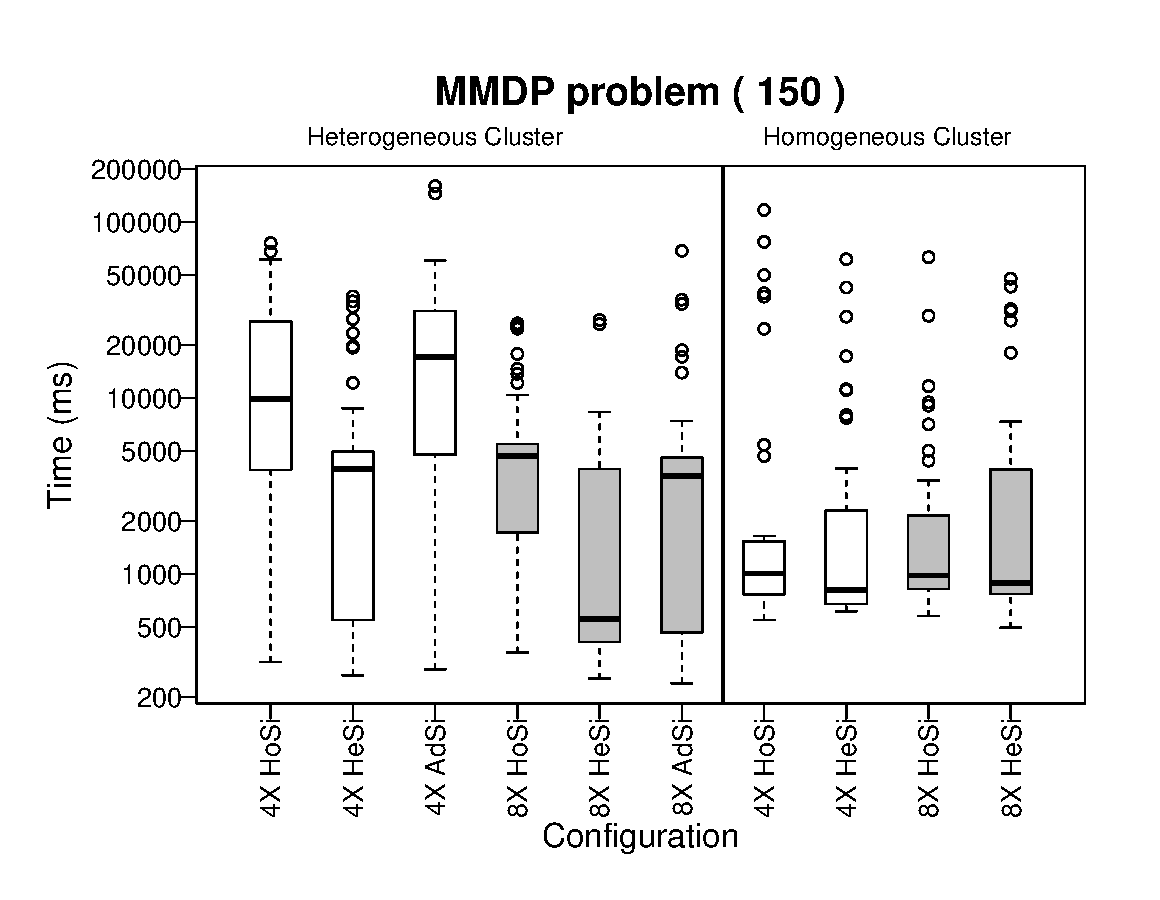
\includegraphics[width =6.5cm] {MMDP_150_TIME.eps}
   \label{subfig:150time}
}
\subfigure[]{
    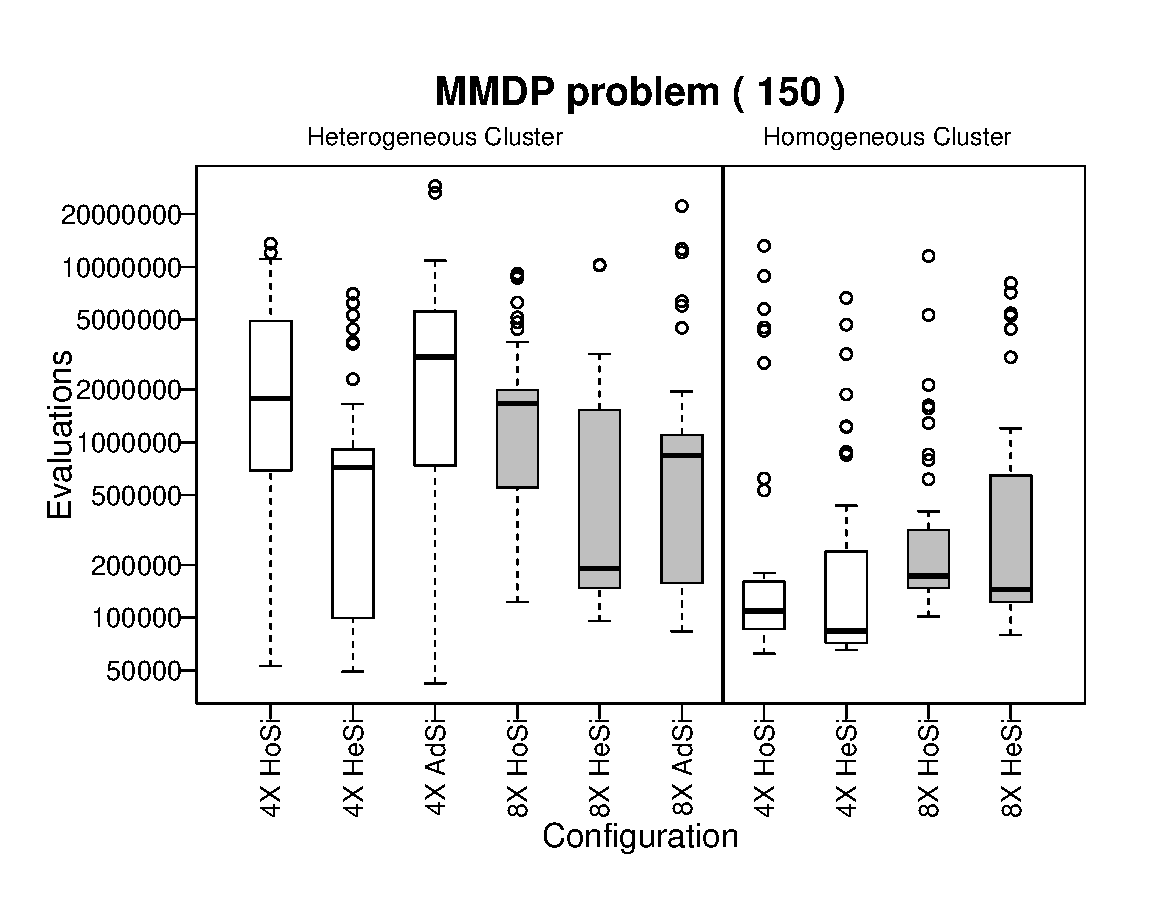
\includegraphics[width =6.5cm] {MMDP_150_EVALS.eps}
   \label{subfig:150evals}
}
\subfigure[]{
    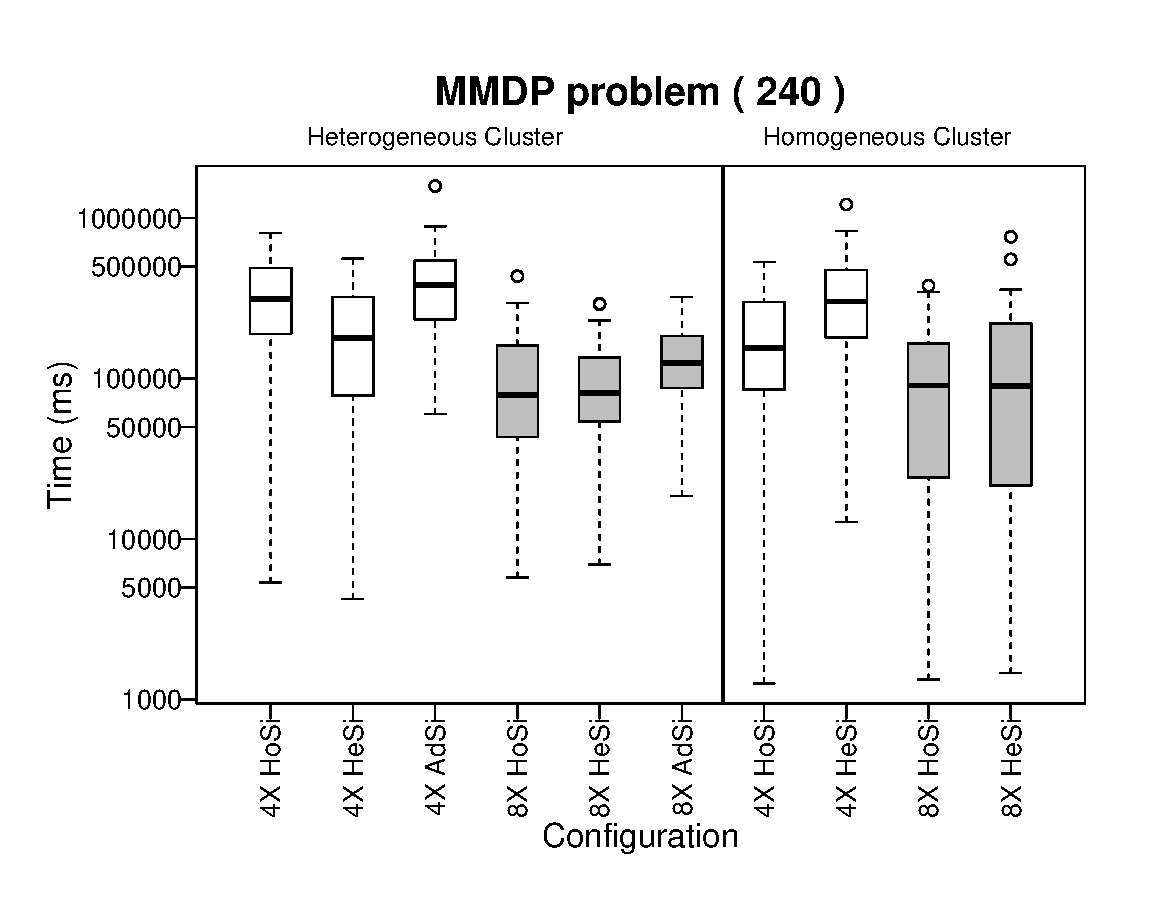
\includegraphics[width =6.5cm] {MMDP_240_TIME.eps}
   \label{subfig:240time}
}
\subfigure[]{
    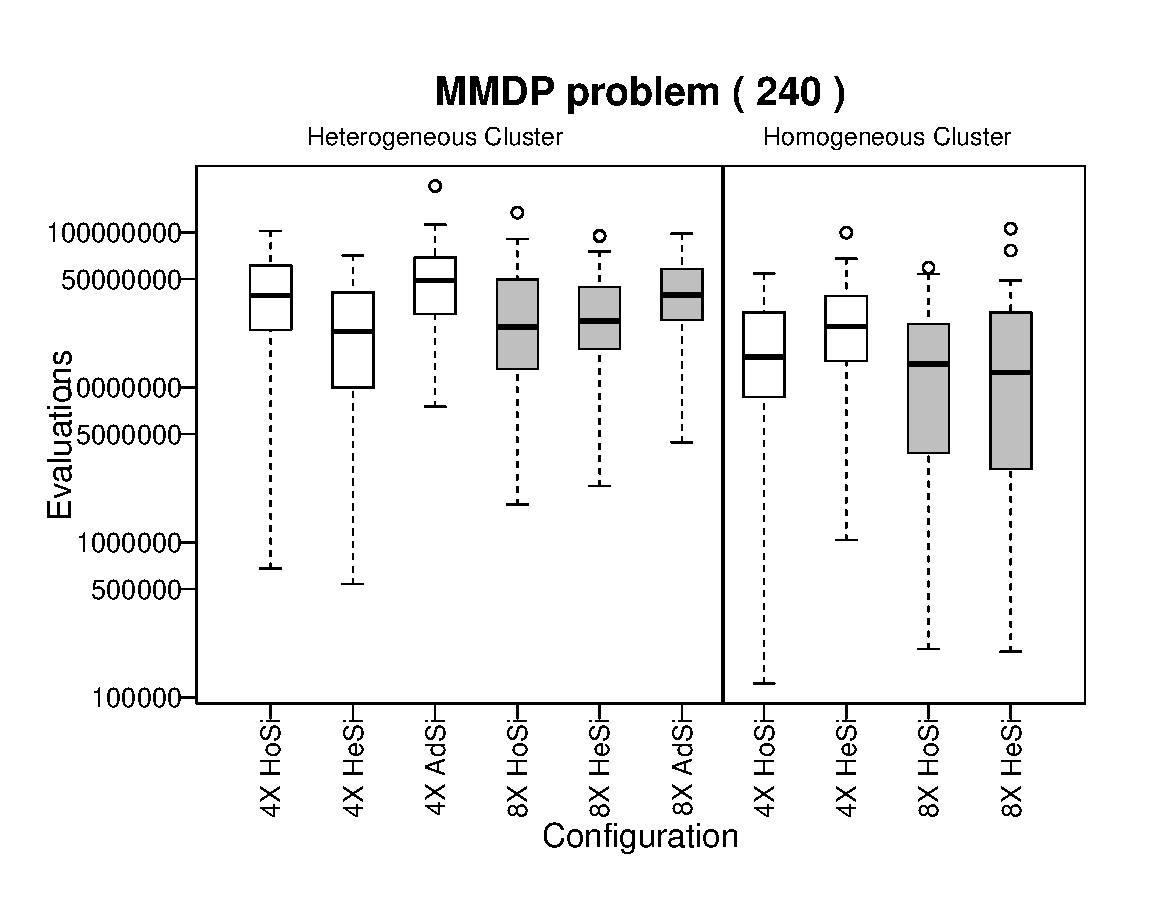
\includegraphics[width =6.5cm] {MMDP_240_EVALS.eps}
   \label{subfig:240evals}
}

\subfigure[]{
    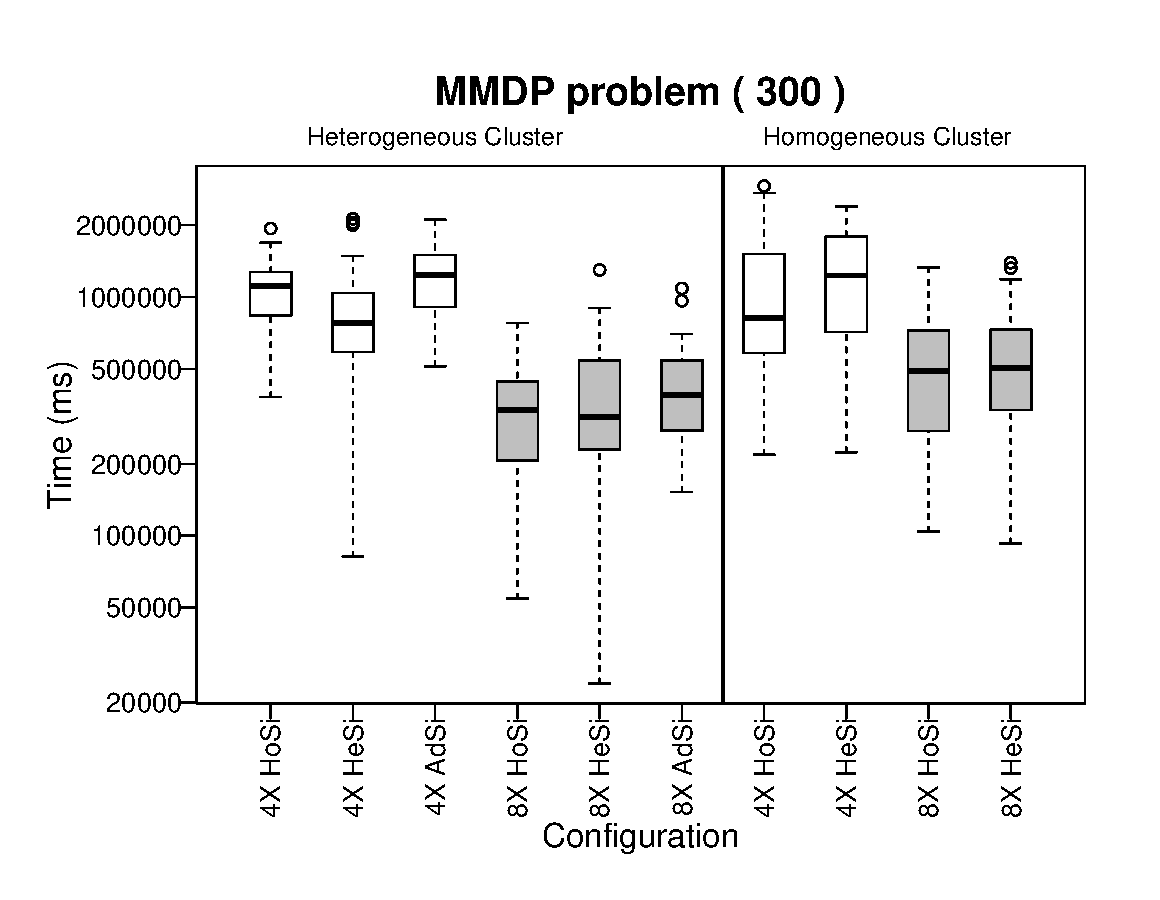
\includegraphics[width =6.5cm] {MMDP_300_TIME.eps}
    \label{subfig:300time}
}
\subfigure[]{
    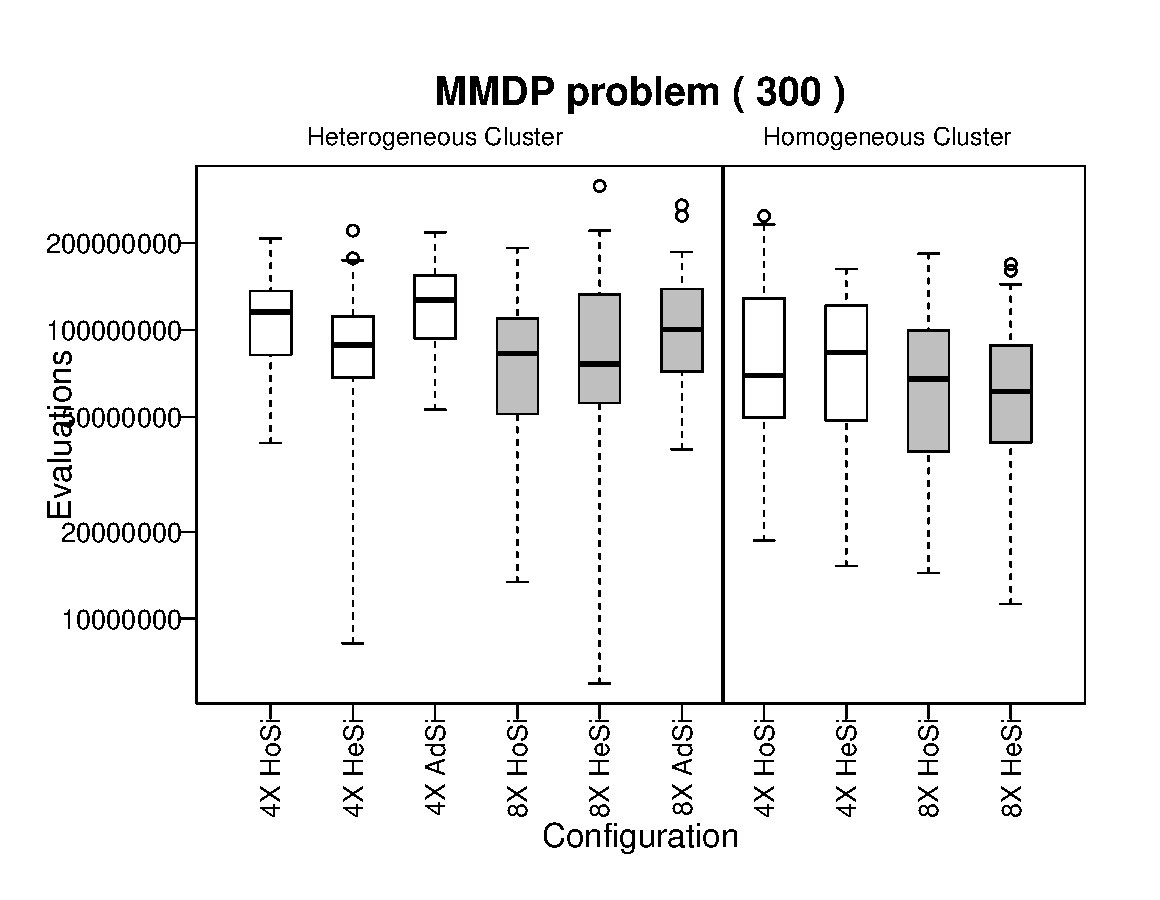
\includegraphics[width =6.5cm] {MMDP_300_EVALS.eps}
    \label{subfig:300evals}
}
\caption{Time (ms) and evaluations needed to obtain the optimum for the MMDP problem. White colour is 4X and grey colour is 8X.}
\label{fig:boxplotsMMDP}
\end{figure}











%%%%%ONEMAX

\begin{figure}[htb]
\centering
\subfigure[]{
    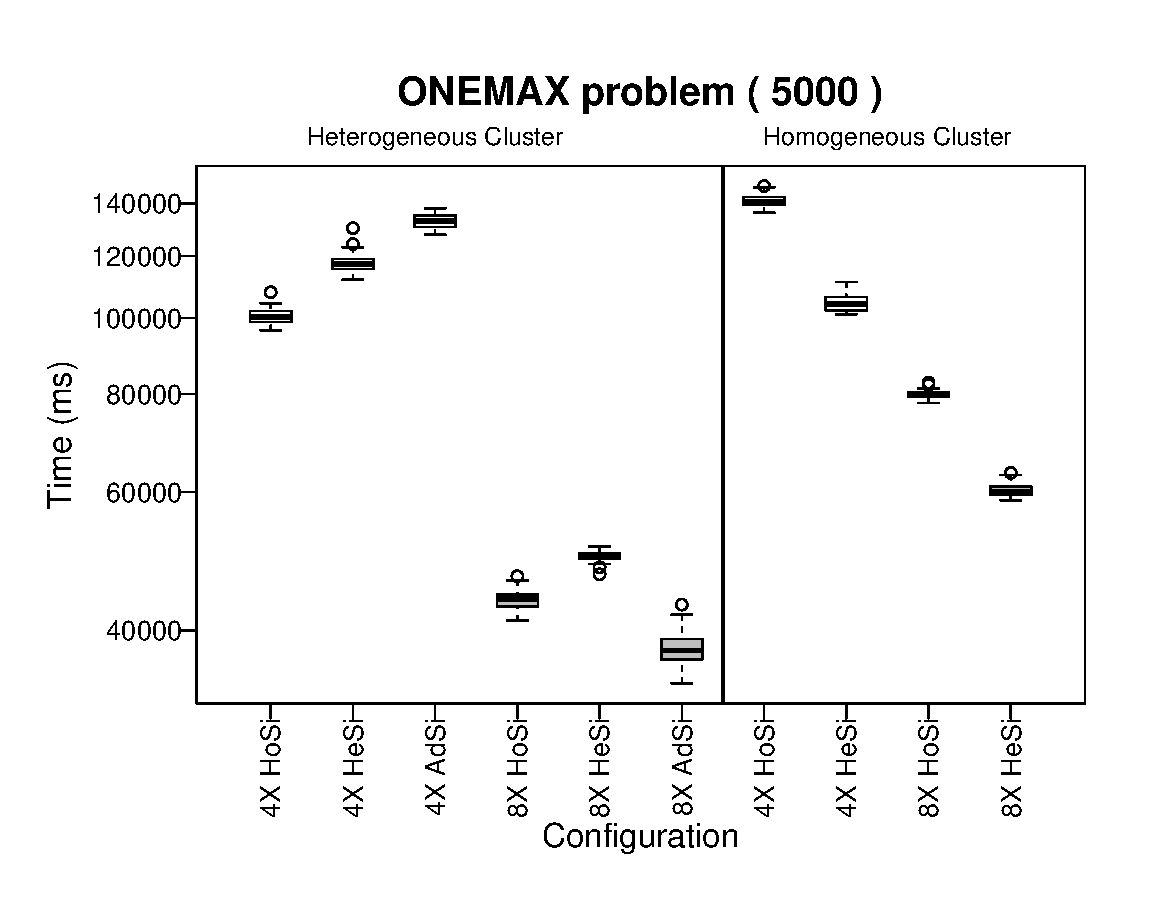
\includegraphics[width =6.5cm] {ONEMAX_5000_TIME.eps}
   \label{subfig:5000time}
}
\subfigure[]{
    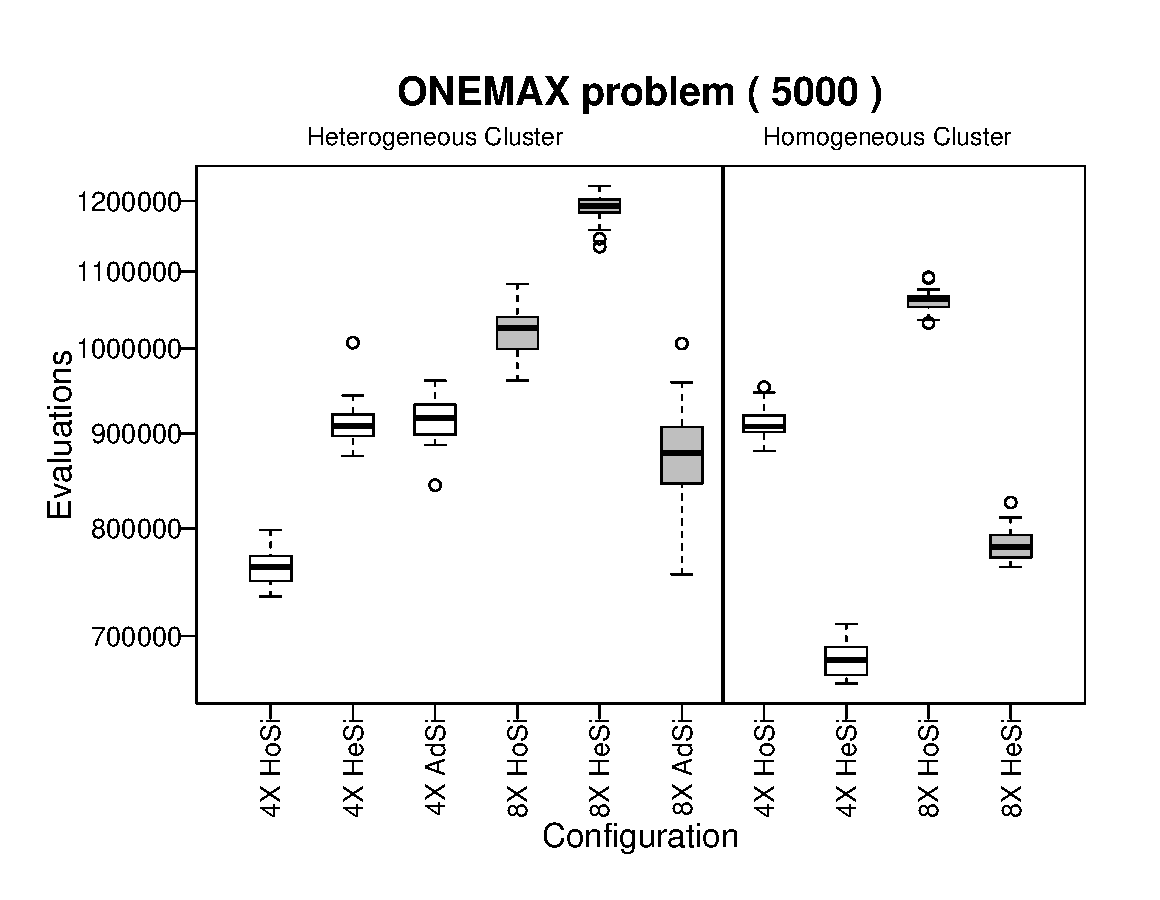
\includegraphics[width =6.5cm] {ONEMAX_5000_EVALS.eps}
   \label{subfig:5000evals}
}
\subfigure[]{
    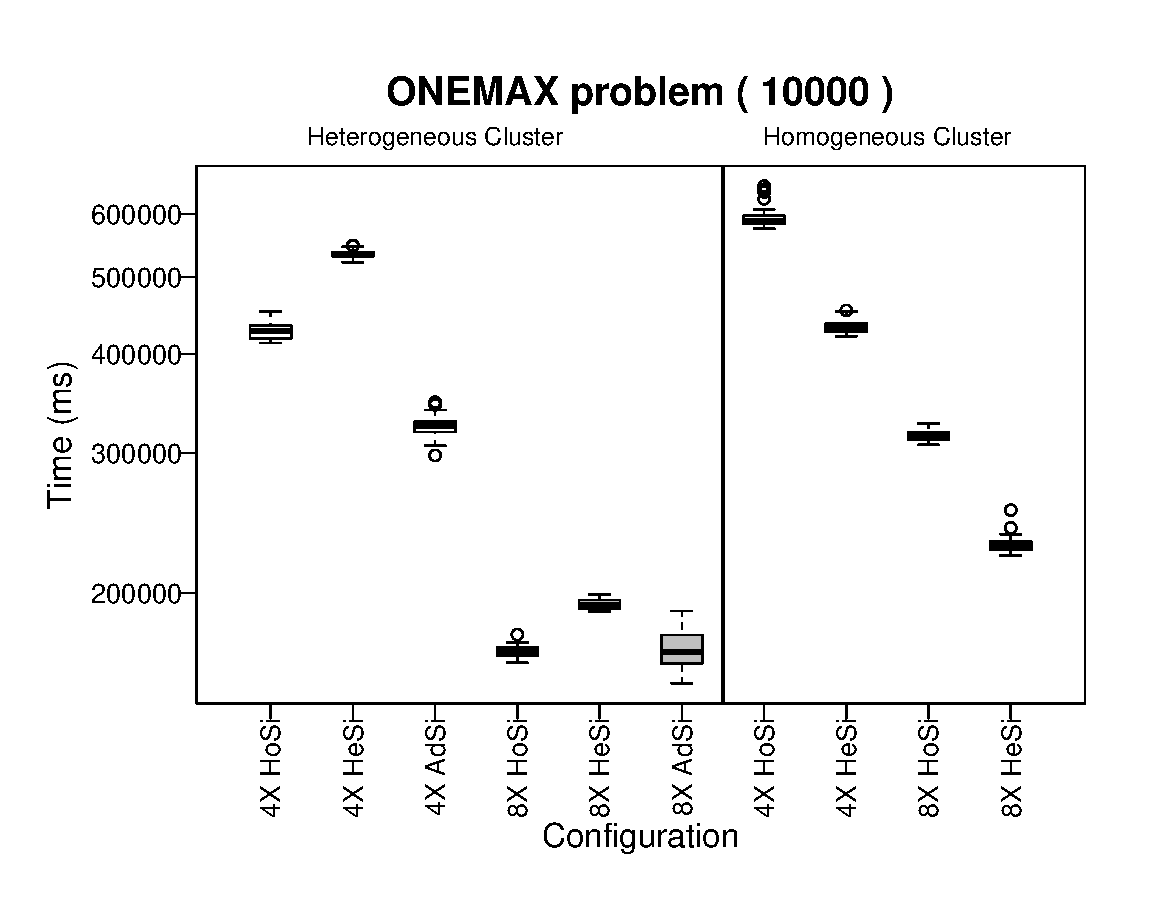
\includegraphics[width =6.5cm] {ONEMAX_10000_TIME.eps}
   \label{subfig:10000time}
}
\subfigure[]{
    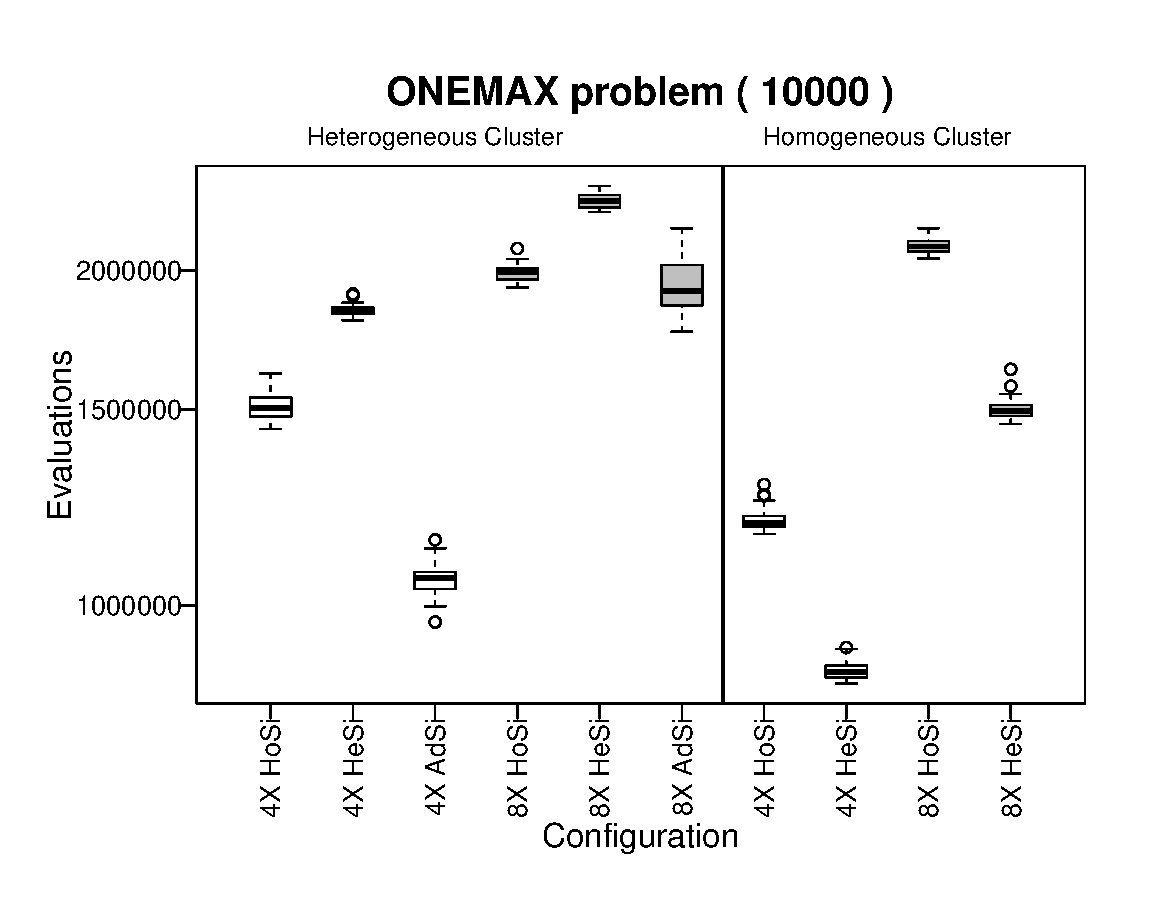
\includegraphics[width =6.5cm] {ONEMAX_10000_EVALS.eps}
   \label{subfig:10000evals}
}

\subfigure[]{
    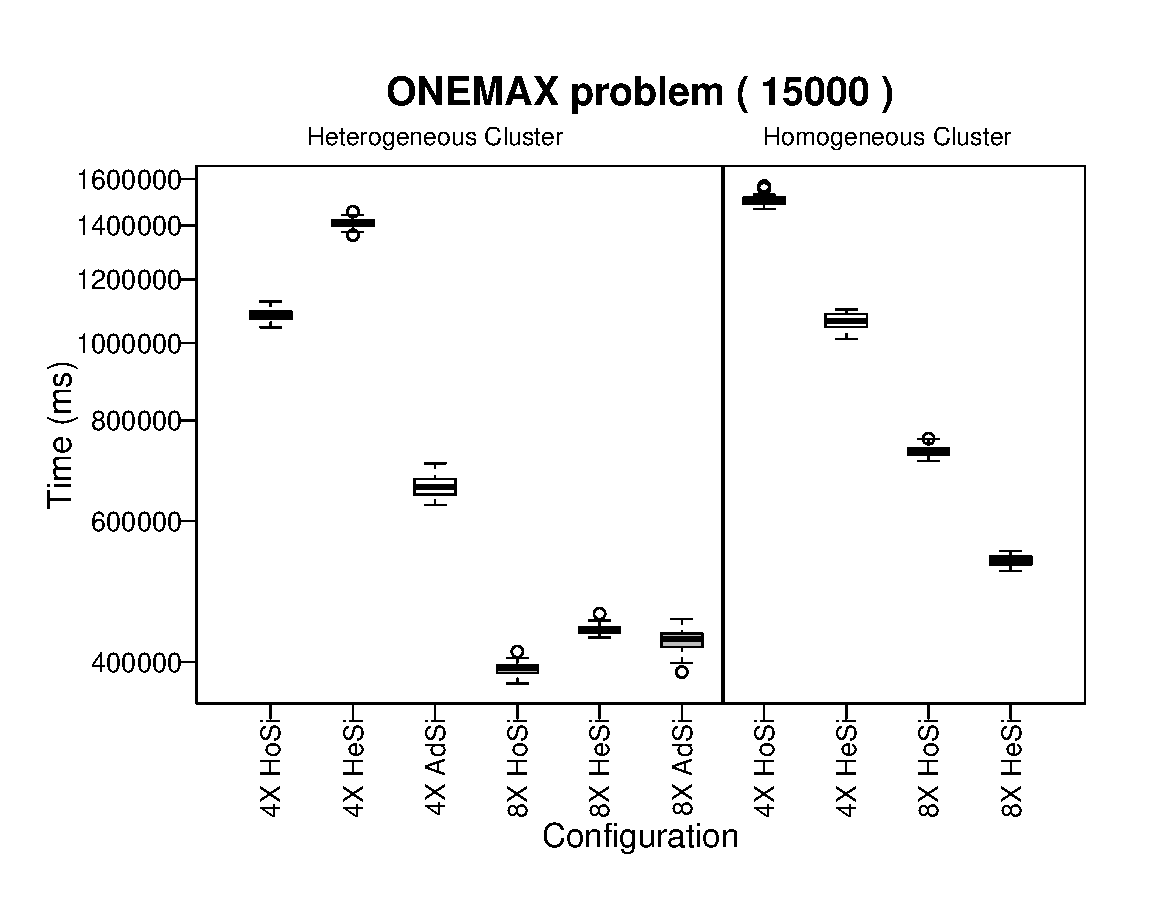
\includegraphics[width =6.5cm] {ONEMAX_15000_TIME.eps}
    \label{subfig:15000time}
}
\subfigure[]{
    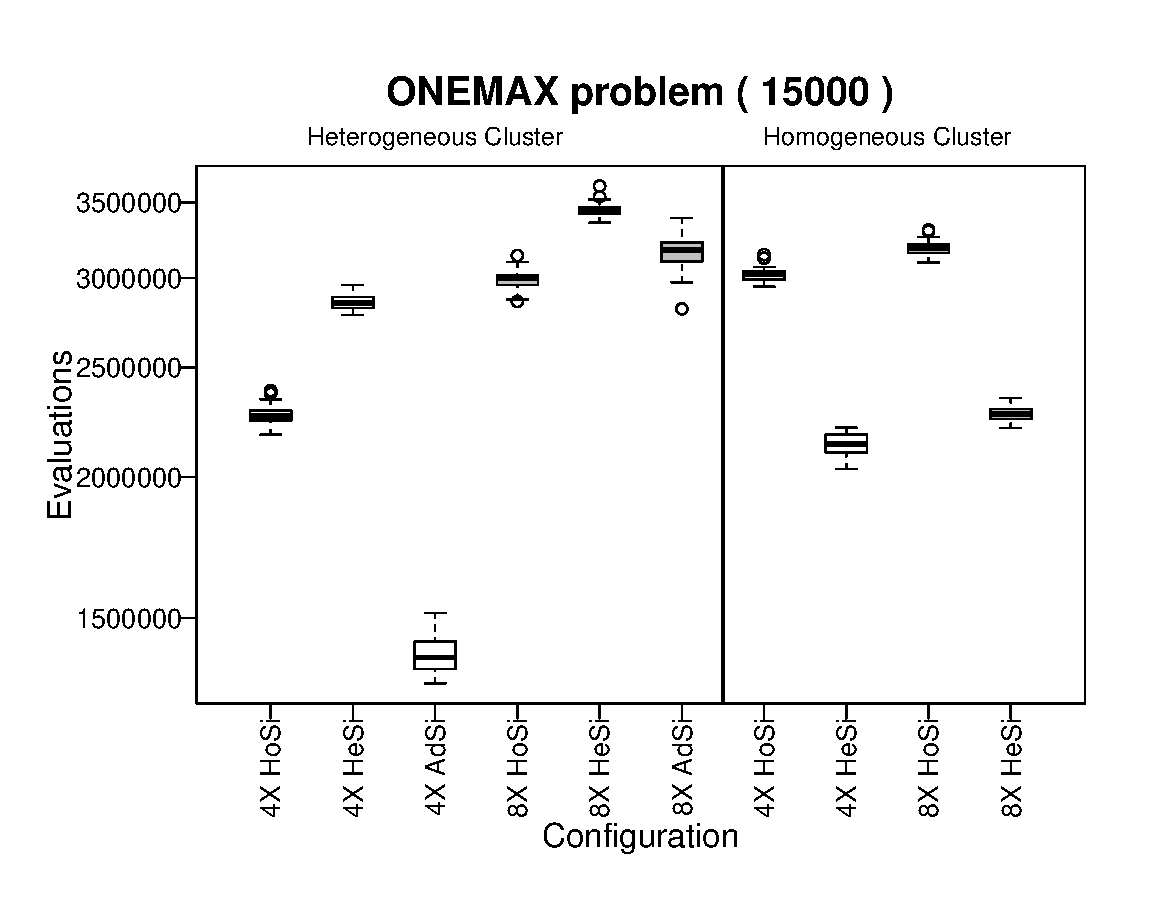
\includegraphics[width =6.5cm] {ONEMAX_15000_EVALS.eps}
    \label{subfig:15000evals}
}
\caption{Time (ms) and evaluations needed to obtain the optimum for the OneMax problem. White colour is 4X and grey colour is 8X.}
\label{fig:boxplotsONEMAX}
\end{figure}


%%ROSENBROCK
\begin{figure}[htb]
\centering
\subfigure[]{
    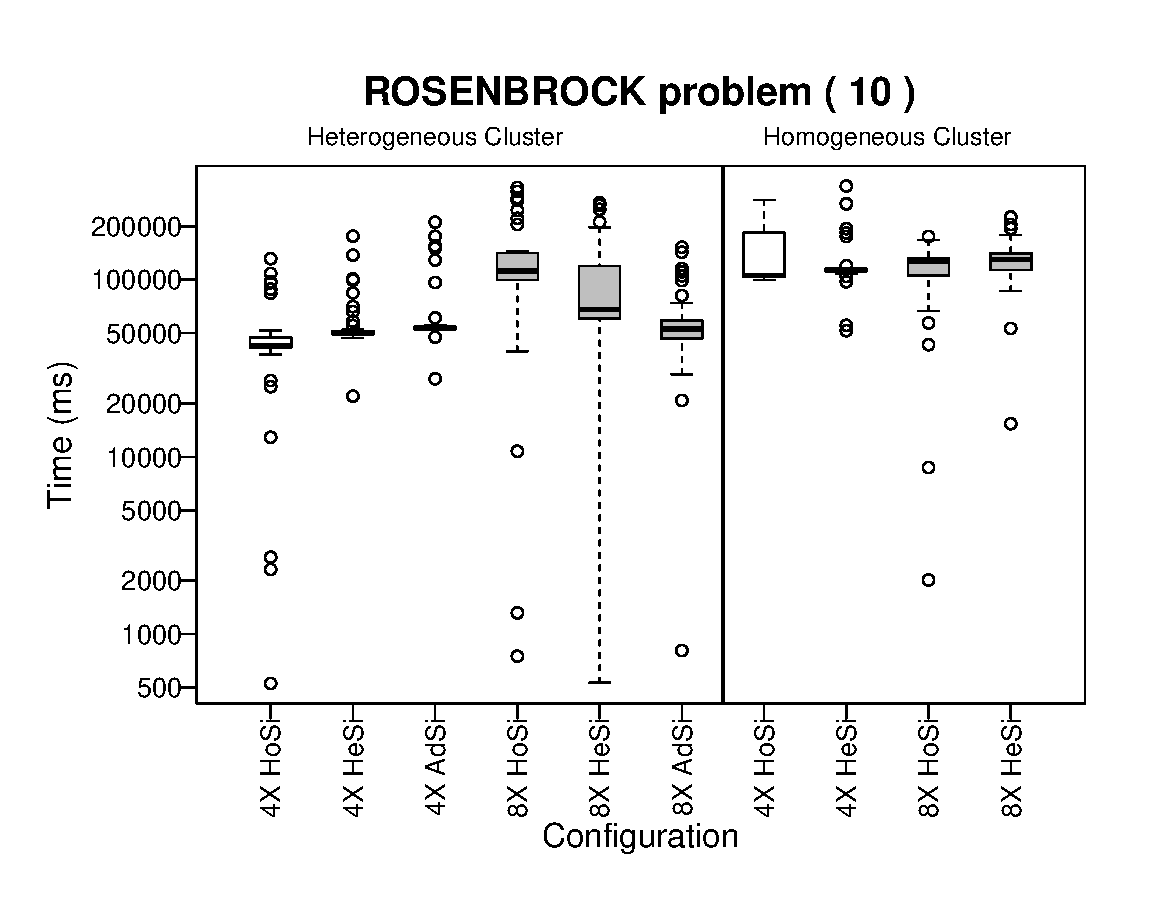
\includegraphics[width =6.5cm] {ROSENBROCK_10_TIME.eps}
   \label{subfig:10time}
}
\subfigure[]{
    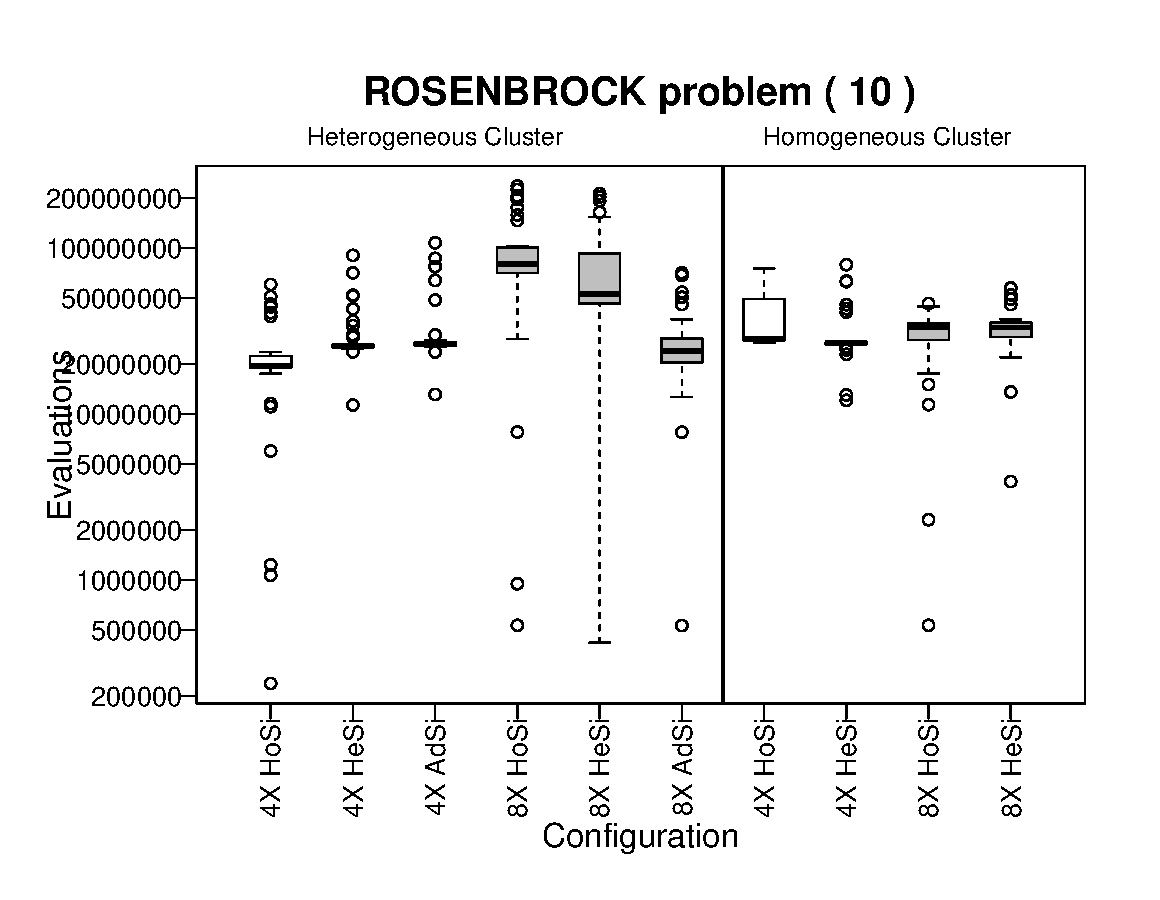
\includegraphics[width =6.5cm] {ROSENBROCK_10_EVALS.eps}
   \label{subfig:10evals}
}
\subfigure[]{
    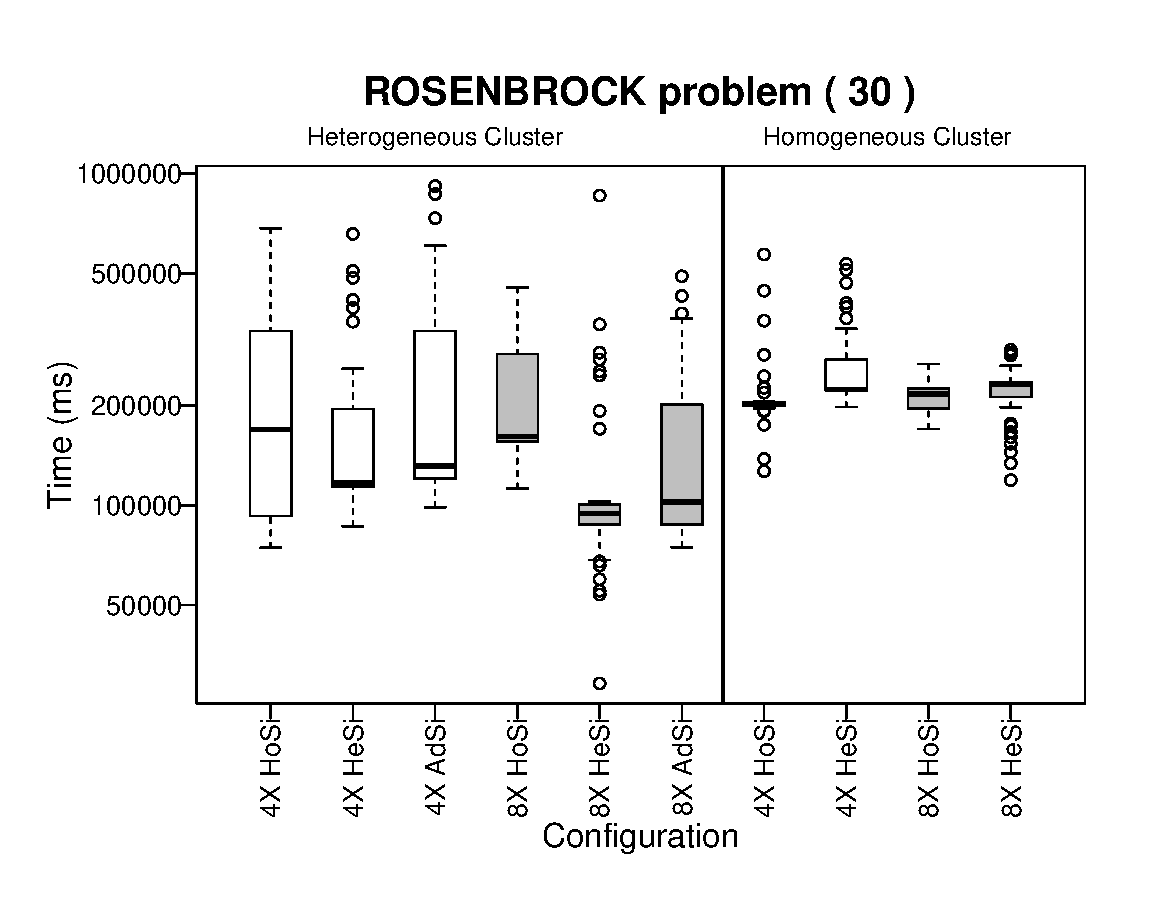
\includegraphics[width =6.5cm] {ROSENBROCK_30_TIME.eps}
   \label{subfig:30time}
}
\subfigure[]{
    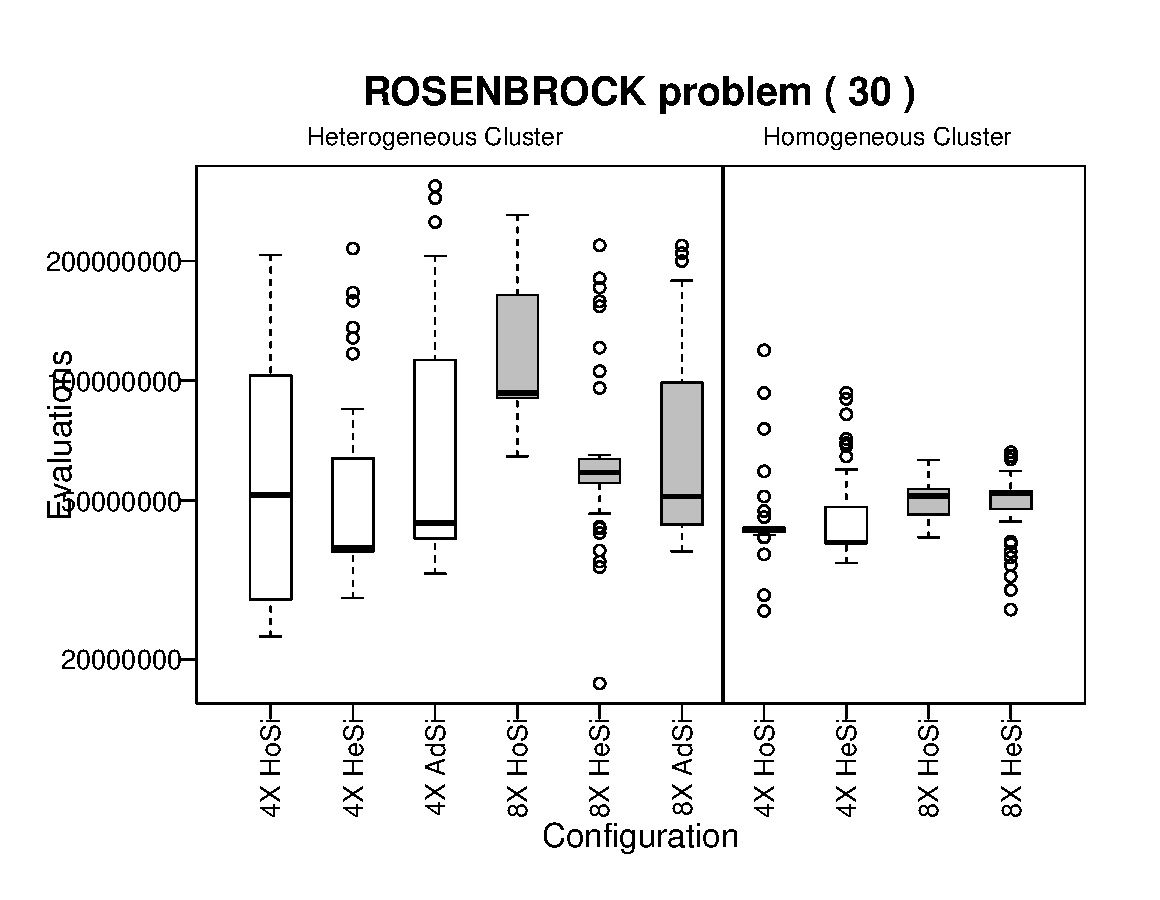
\includegraphics[width =6.5cm] {ROSENBROCK_30_EVALS.eps}
   \label{subfig:30evals}
}

\subfigure[]{
    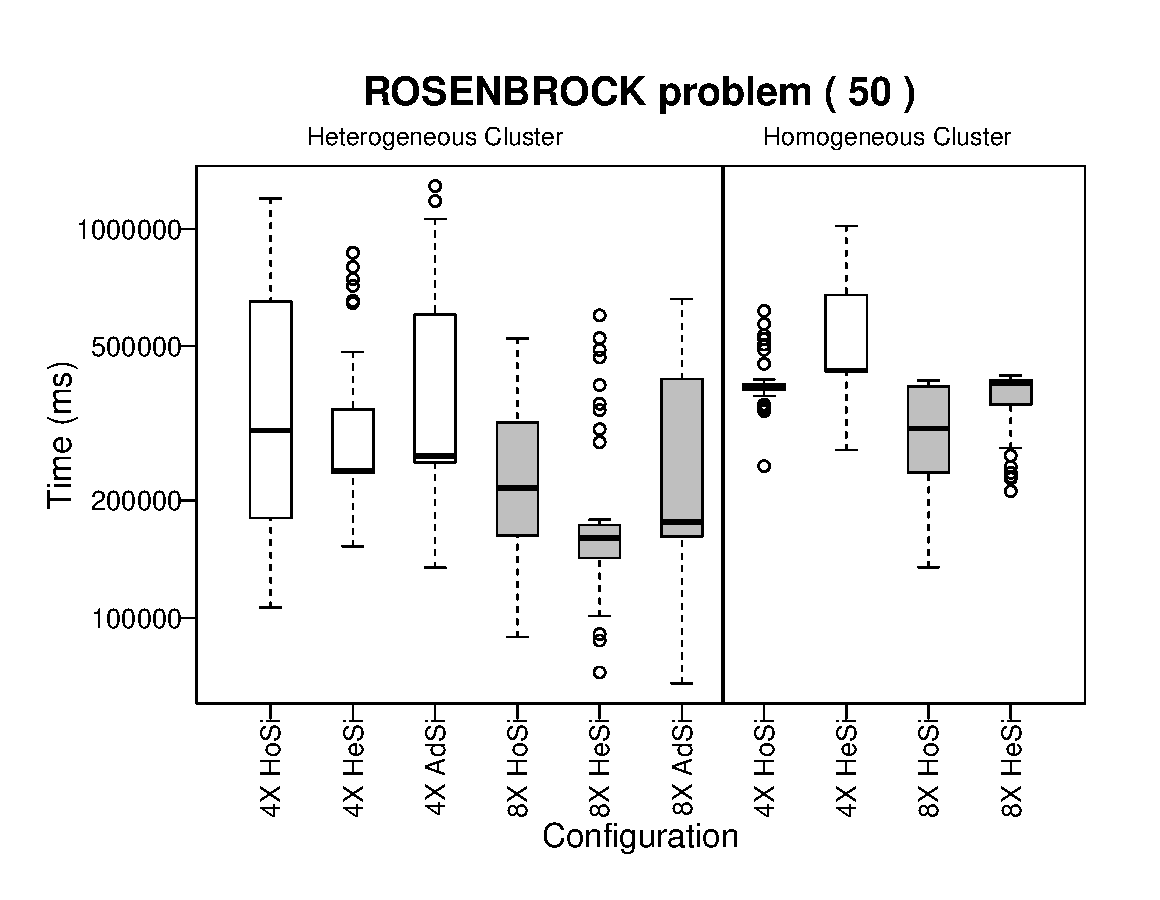
\includegraphics[width =6.5cm] {ROSENBROCK_50_TIME.eps}
    \label{subfig:50time}
}
\subfigure[]{
    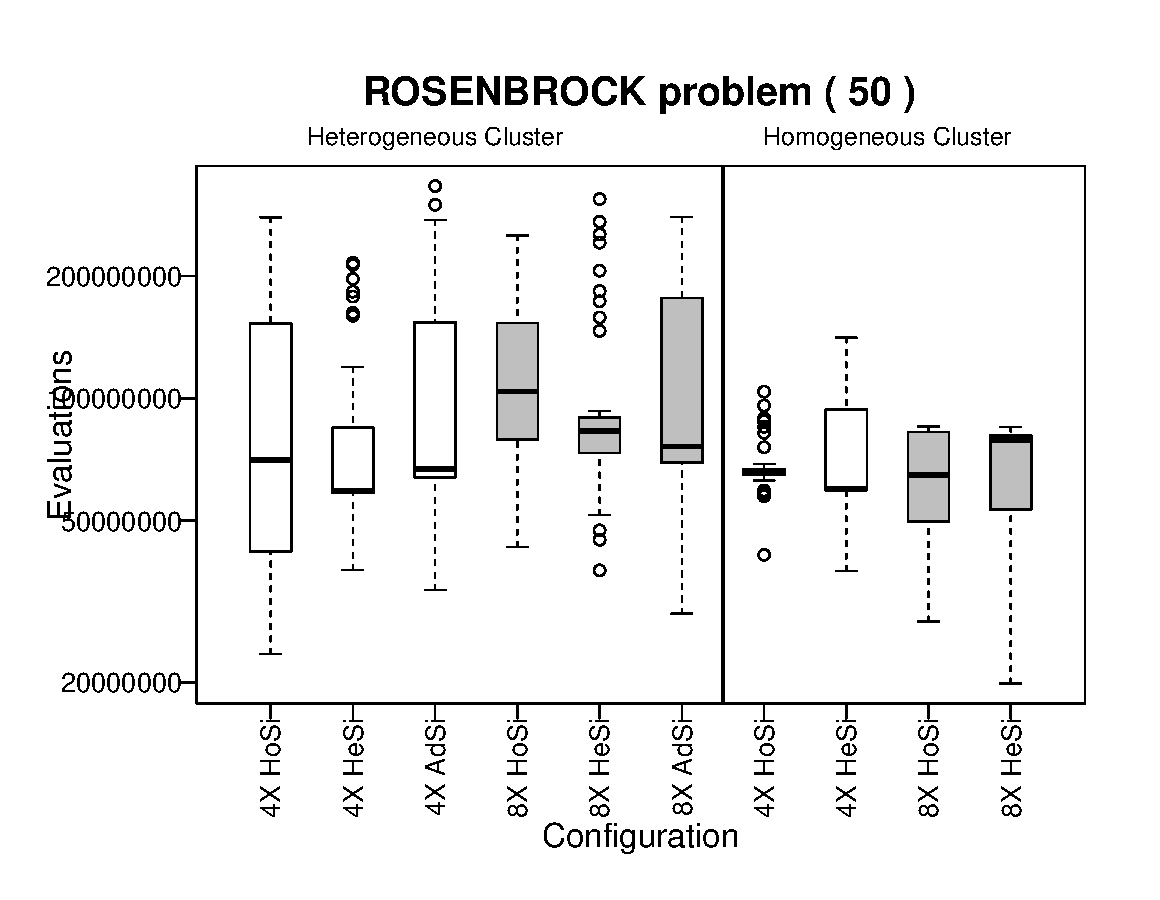
\includegraphics[width =6.5cm] {ROSENBROCK_50_EVALS.eps}
    \label{subfig:50evals}
}
\caption{Time (ms) and evaluations needed to obtain the optimum for the
  Rosenbrock function problem. White colour is 4X and grey colour is 8X.}

\label{fig:boxplotsROSENBROCK}
\end{figure}




%%%%%%%%%%%%%%%%%%%%%%%GUSTVAO'S GRAPHS %%%%%%%%%%%%%%%%%%%%%%

\begin{figure}[htb]
\centering
\subfigure[150 MMDP HeHW]{
    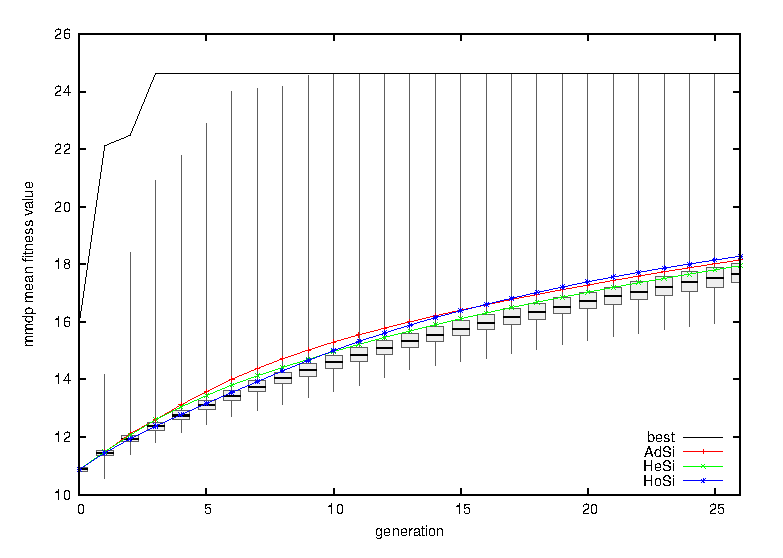
\includegraphics[width =6.5cm] {mmdp-size-150-mut-0.006-xover-1-heterohardware.eps}
   \label{subfig:graph150MMDPHeHW}
}
\subfigure[150 MMDP HoHW]{
    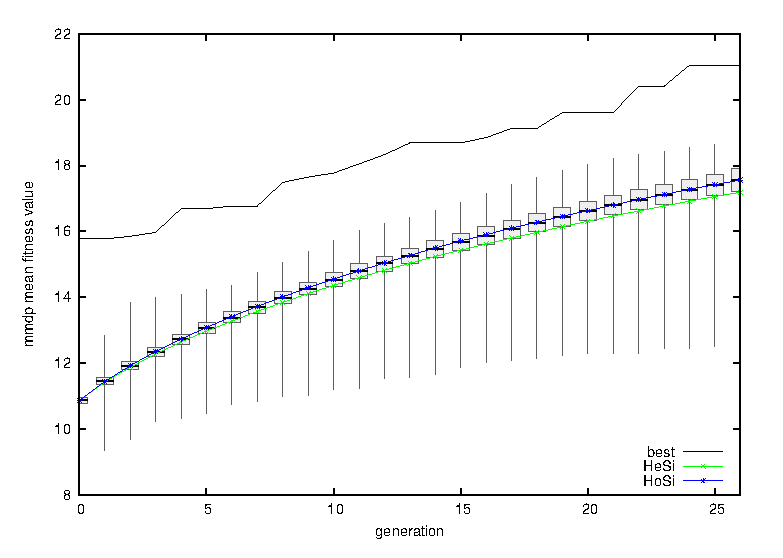
\includegraphics[width =6.5cm] {mmdp-size-150-mut-0.006-xover-1-homohardware.eps}
   \label{subfig:graph150MMDPHoHW}
}
\subfigure[240 MMDP HeHW]{
    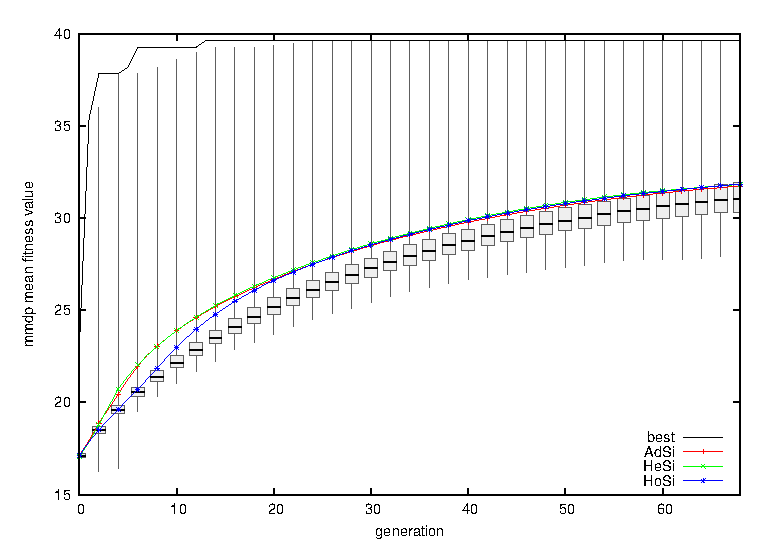
\includegraphics[width =6.5cm] {mmdp-size-240-mut-0.004-xover-1-heterohardware.eps}
   \label{subfig:graph240MMDPHeHW}
}
\subfigure[240 MMDP HoHW]{
    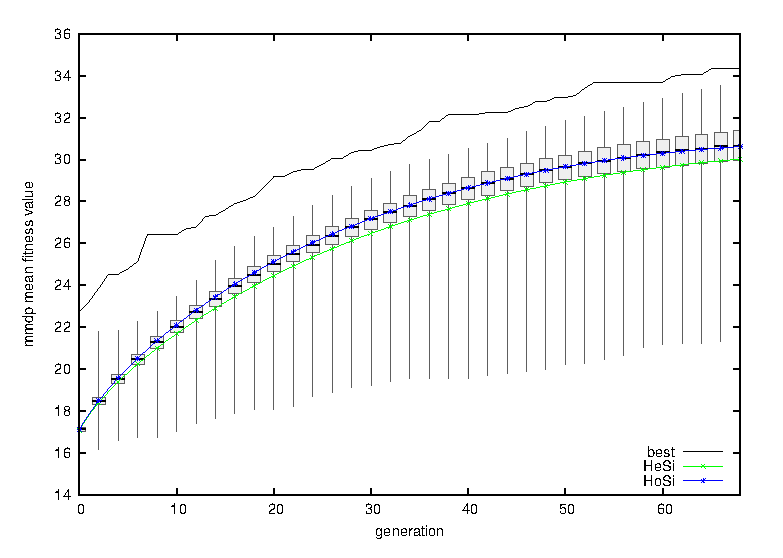
\includegraphics[width =6.5cm] {mmdp-size-240-mut-0.004-xover-1-homohardware.eps}
   \label{subfig:graph240MMDPHoHW}
}

\subfigure[300 MMDP HeHW]{
    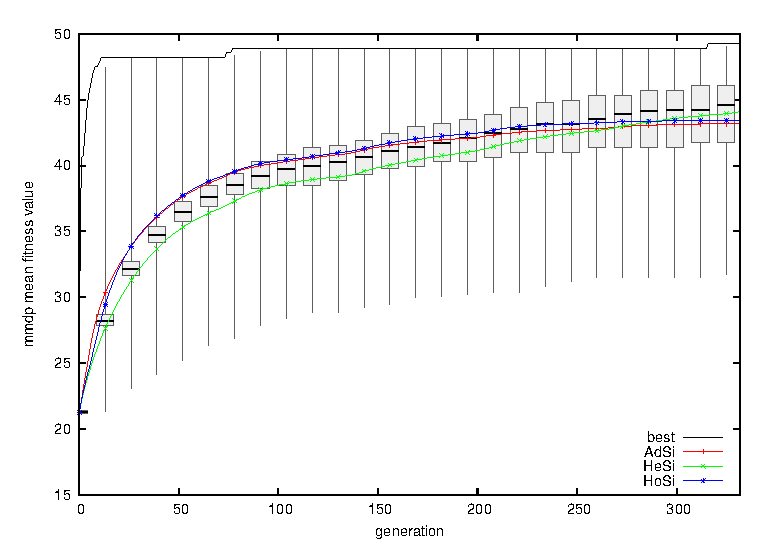
\includegraphics[width =6.5cm] {mmdp-size-300-mut-0.003-xover-1-heterohardware.eps}

   \label{subfig:graph300MMDPHeHW}
}
\subfigure[300 MMDP HoHW]{
    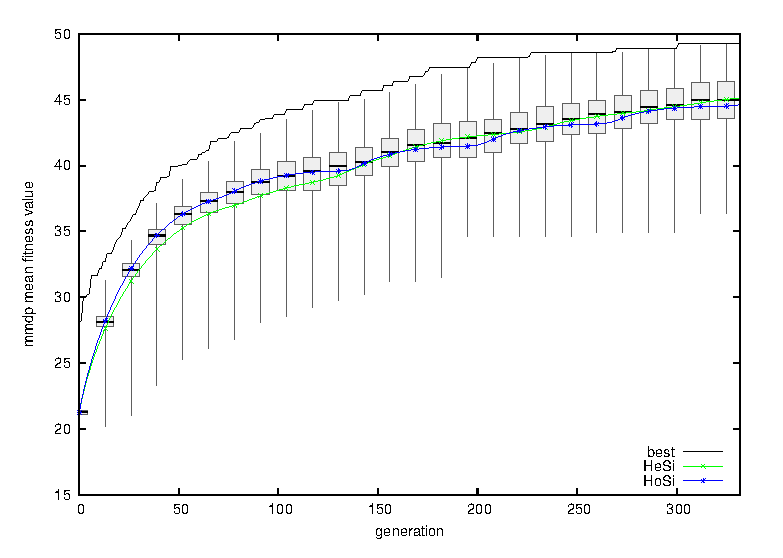
\includegraphics[width =6.5cm] {mmdp-size-300-mut-0.003-xover-1-homohardware.eps}
    \label{subfig:graph300MMDPHoHW}
}
\caption{Average fitness value along the evolution of the individuals for MMDP problem in 8X/HeHW and 8X/HoHW.}
\label{fig:graphsMMDP}
\end{figure}











%%%%%ONEMAX
\begin{figure}[htb]
\centering
\subfigure[5000 ONEMAX HeHW]{
    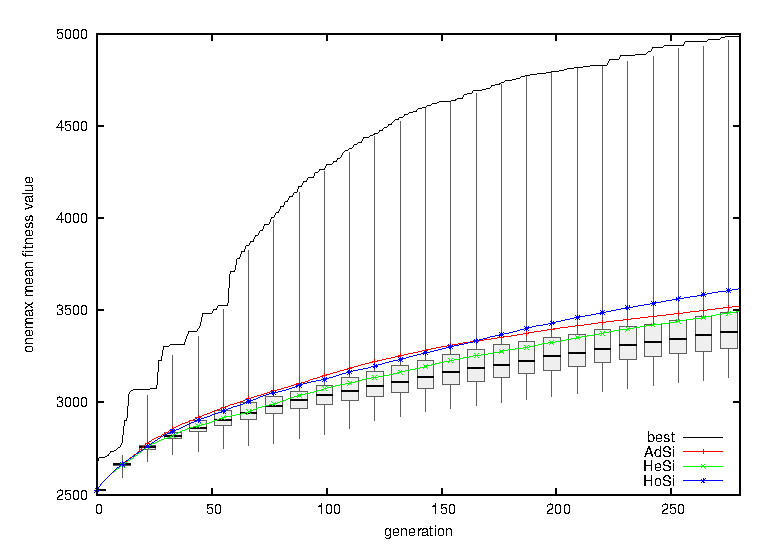
\includegraphics[width =6.5cm] {onemax-size-5000-mut-0.0002-xover-1-heterohardware.eps}
   \label{subfig:graph150ONEMAXHeHW}
}
\subfigure[5000 ONEMAX HoHW]{
    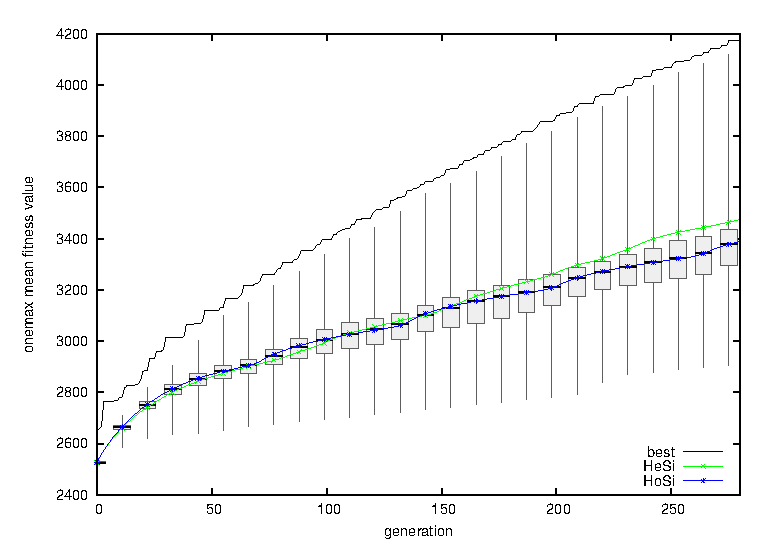
\includegraphics[width =6.5cm] {onemax-size-5000-mut-0.0002-xover-1-homohardware.eps}
   \label{subfig:graph150ONEMAXHoHW}
}
\subfigure[10000 ONEMAX HeHW]{
    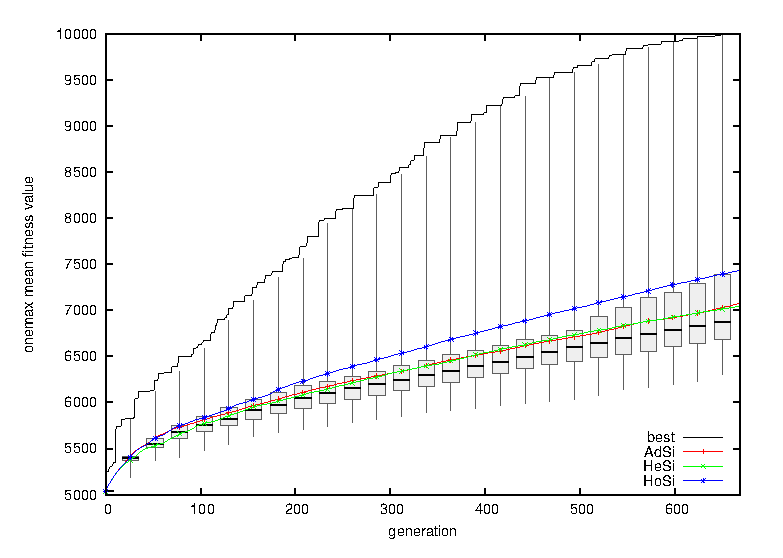
\includegraphics[width =6.5cm] {onemax-size-10000-mut-0.0001-xover-1-heterohardware.eps}
   \label{subfig:graph150ONEMAXHoHW}
}
\subfigure[10000 ONEMAX HoHW]{
    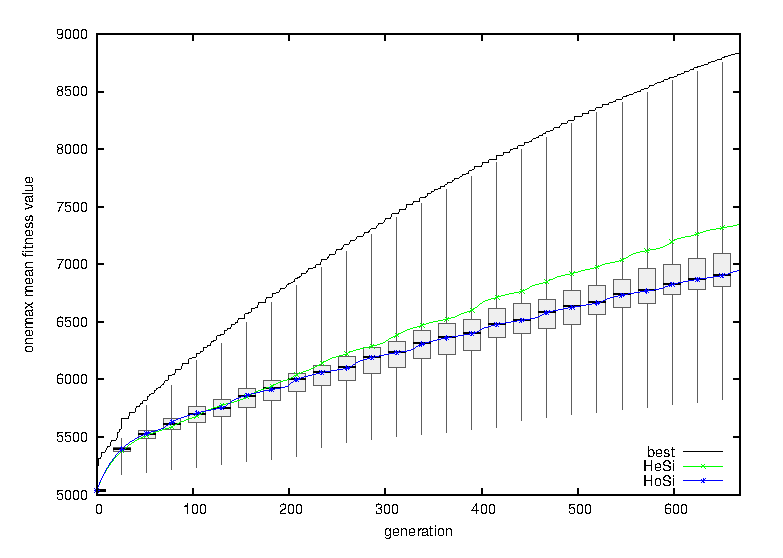
\includegraphics[width =6.5cm] {onemax-size-10000-mut-0.0001-xover-1-homohardware.eps}
   \label{subfig:graph240ONEMAXHoHW}
}

\subfigure[15000 ONEMAX HeHW]{
    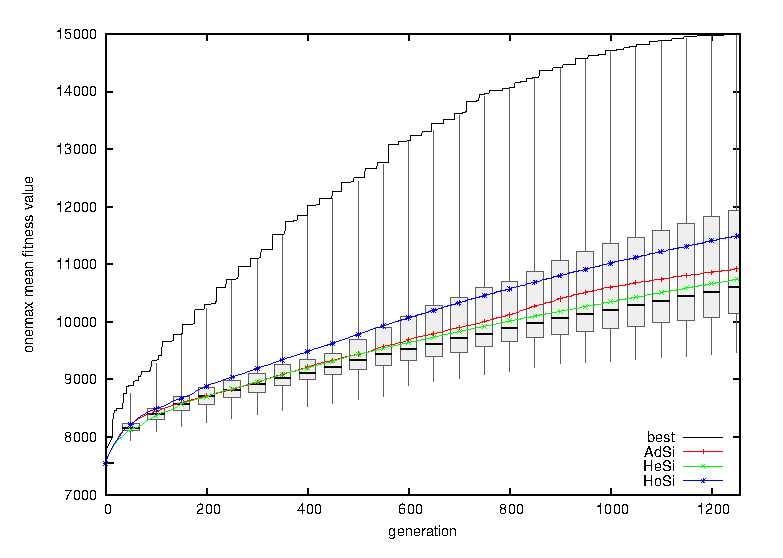
\includegraphics[width =6.5cm] {onemax-size-15000-mut-0.00006-xover-1-heterohardware.eps}

   \label{subfig:graph300ONEMAXHeHW}
}
\subfigure[15000 ONEMAX HoHW]{
    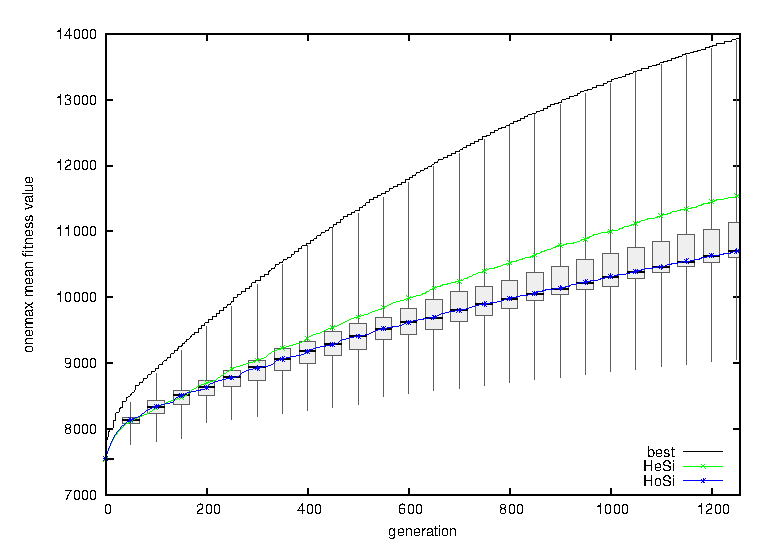
\includegraphics[width =6.5cm] {onemax-size-15000-mut-0.00006-xover-1-homohardware.eps}
    \label{subfig:graph300ONEMAXHoHW}
}
\caption{Average fitness value along the evolution of the individuals for ONEMAX problem in 8X/HeHW and 8X/HoHW.}
\label{fig:graphsONEMAX}
\end{figure}








%%%%%ROSENBROCK
\begin{figure}[htb]
\centering
\subfigure[10 ROSENBROCK HeHW]{
    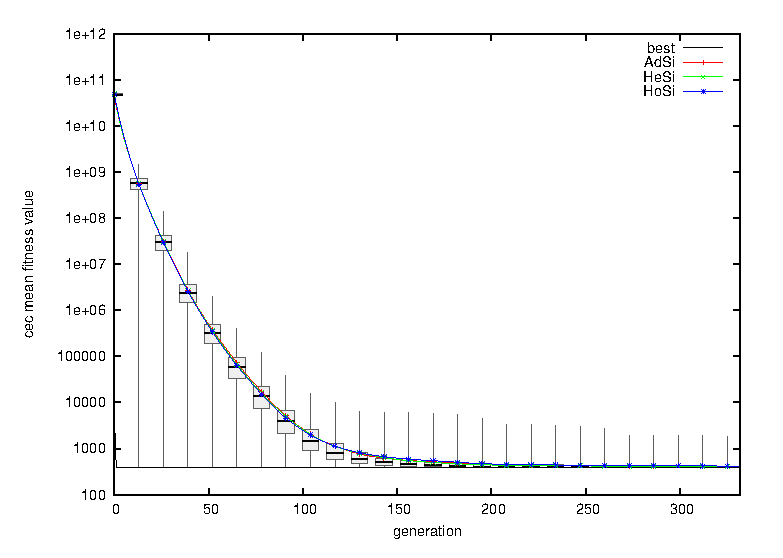
\includegraphics[width =6.5cm] {cec-size-10-mut-0.1-xover-1-heterohardware.eps}
   \label{subfig:graph10ROSENBROCKHeHW}
}
\subfigure[10 ROSENBROCK HoHW]{
    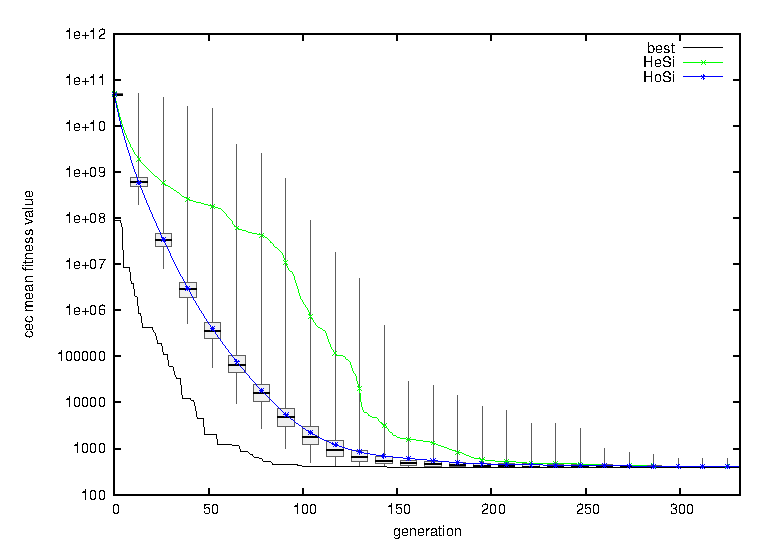
\includegraphics[width =6.5cm] {cec-size-10-mut-0.1-xover-1-homohardware.eps}
   \label{subfig:graph10ROSENBROCKHoHW}
}
\subfigure[30 ROSENBROCK HeHW]{
    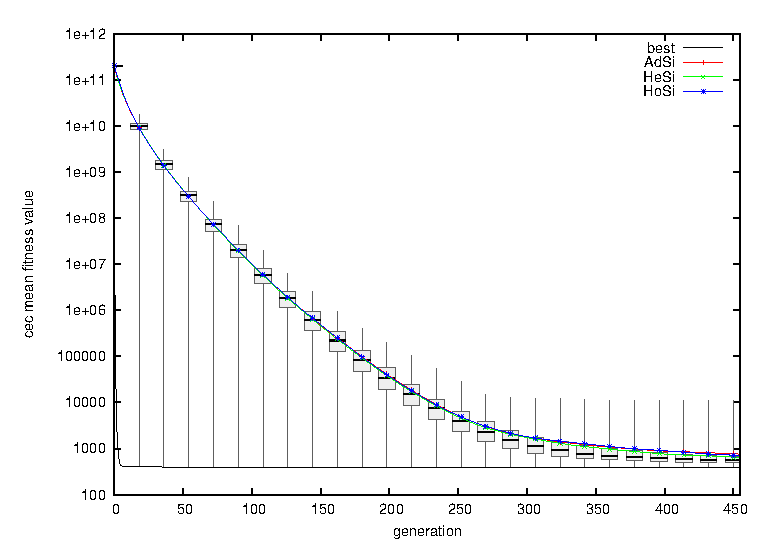
\includegraphics[width =6.5cm] {cec-size-30-mut-0.03-xover-1-heterohardware.eps}
   \label{subfig:graph30ROSENBROCKHeHW}
}
\subfigure[30 ROSENBROCK HoHW]{
    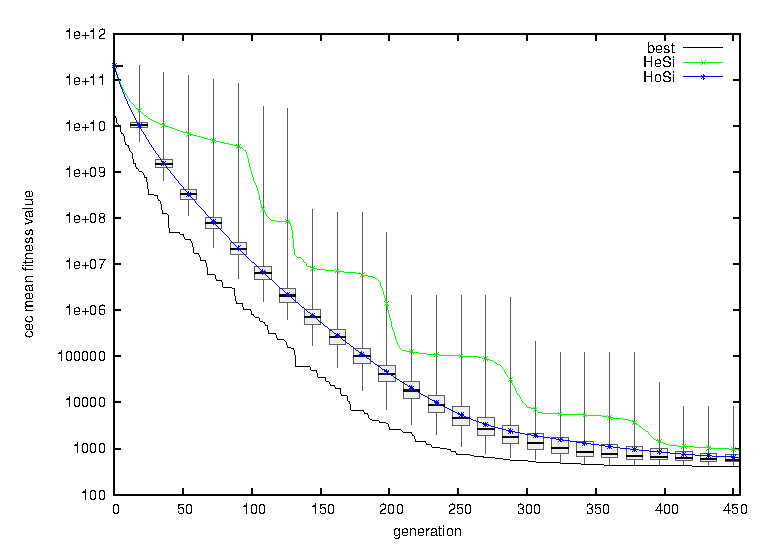
\includegraphics[width =6.5cm] {cec-size-30-mut-0.03-xover-1-homohardware.eps}
   \label{subfig:graph30ROSENBROCKHoHW}
}

\subfigure[50 ROSENBROCK HeHW]{
    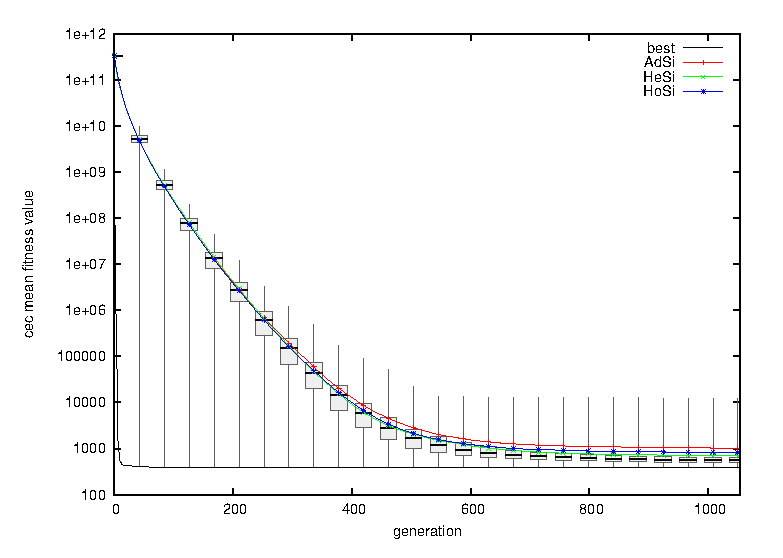
\includegraphics[width =6.5cm] {cec-size-50-mut-0.02-xover-1-heterohardware.eps}

   \label{subfig:graph50ROSENBROCKHeHW}
}
\subfigure[50 ROSENBROCK HoHW]{
    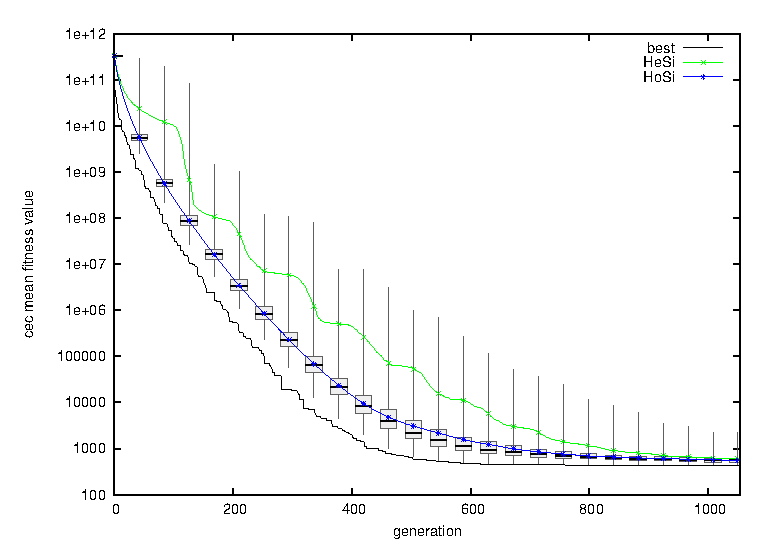
\includegraphics[width =6.5cm] {cec-size-50-mut-0.02-xover-1-homohardware.eps}
    \label{subfig:graph50ROSENBROCKHoHW}
}
\caption{Average fitness value along the evolution of the individuals for ROSENBROCK problem in 8X/HeHW and 8X/HoHW.}
\label{fig:graphsROSENBROCK}
\end{figure}



Obtained results, grouped by problem, are also plotted in the boxplots of Figures \ref{fig:boxplotsMMDP}, \ref{fig:boxplotsONEMAX} and \ref{fig:boxplotsROSENBROCK}, for a better understanding of the behaviour of each configuration. To show the evolution in each configuration the average population fitness during all the runs has been plotted using boxplots into evolution graphs, with the best individual of all the runs and the average fitness of each method (Figures \ref{fig:graphsMMDP}, \ref{fig:graphsONEMAX} and \ref{fig:graphsROSENBROCK}). 
Only the 8X graphics have been shown in order to not extend too much the paper extension. 

The results show that, in general, there are significant differences
depending on the problem, configuration or number of nodes. Also, it
can be seen that the number of evaluations may not be a good indicator
when comparing heterogeneous environments. For example, for the OneMax
problem (Figure \ref{fig:boxplotsONEMAX}), using 8 nodes instead of 4,
requires more evaluations to finish, and yet, less time to achieve the
optimum.  
Also, the average amount of time needed to solve the problems may vary
in larger ranges for MMDP and Rosenbrock. This can explain the different results
among the problems.  

At first glance, and as expected \cite{Wolpert97NFL}, fitting the
population sub-sizes to heterogeneous clusters does not always imply an
improvement in time. The HeSi parameter setting can improve time in
the MMDP and Rosenbrock for HeHW, but in case of the OneMax problem,
offline fitting  the sub-population sizes significantly increases  the running time for solving it in the heterogeneous cluster. This can be seen in the average evolution of the OneMax problem in Figure \ref{fig:graphsONEMAX}. In all HeHW configurations the average fitness of the population is located in the lower parts of the boxplots with respect to the best fitness, while in the HoHW the evolution is closer to this value. The HeSi and HoSi lines are always moving closer during all the evolution, while the AdSi is obtaining better results at the same time. Also, the best individual of all runs (black line) does not converge as smoothly as in HoHW.
This can be explained because the efficiency on OneMax problem depends mainly on the ability to mix
the building-blocks, and less on the genetic diversity and size of the
population (as with MMDP or Rosenbrock). A high genetic diversity is not particularly
required. When properly tuned, a simple GA is able to solve OneMax in super-linear time, i.e., $l \times log(l)$, with $l$ being the string length \cite{Verma09MapReduce}. Sometimes, problems like OneMax are used
as control functions, in order to check if very efficient algorithms
on hard functions fail on easier ones. 

On the contrary, for the MMDP and Rosenbrock, in the HoHW system,
setting heterogeneous sizes to sub-populations makes no difference in
time, that is, changing this parameter has no influence in the
algorithm's performance. Homogeneous nodes exploring different population sizes at the same speed implies less diversity during the runs. This can be seen in Figures \ref{fig:graphsMMDP} and \ref{fig:graphsROSENBROCK}, where in all the instances of those problems, the average population fitness in HoHW is closer to the best average value attained. This behaviour is opposed to the same problems executed on HeHW, where the difference of the average best fitness and the average population fitness is larger. This difference is  larger at the beginning of the runs (local optima are found faster) but the diversity is still maintained, and being reduced with time.



Finally, the number of nodes affects the behaviour of the
algorithms. In the case of MMDP in the HeHW system, the offline
fitting of the sub-population to the computational  power of each node
makes the algorithm finish significantly earlier in all instances of
the problem in the 4X configuration. However, in the 8X configuration
the time is significantly lower only in the 150 instance. This can be
due to the nature of this problem, as the fitness of the population may stagnate if the optimum is not found on the first steps (see the black line in Figure \ref{fig:graphsMMDP} with respect to the average population fitness boxplots). This behaviour is opposite in the case of the Rosenbrock function, where using a larger number of nodes improves the time with HeSi and AdSi. %TODO



 





Summarising, fitting the population sizes to the
  computational power of each machine (offline and online) can reduce
  the time to obtain the optimum. The same heterogeneous fixed sizes
  in the homogeneous cluster does not produce a significant decrease
  of running time, so the improvement is produced by the heterogeneity
  and not for the different island sizes. 

\subsection{Adaptive sub-population sizes during evolution}

Figure \ref{fig:adaptivesize} shows the average sub-population sizes for each problem of the AdSi/HeHW runs, focusing only on the larger problem instances for the 8X configuration, as the other instances behave in a similar way. These graphics show the average sizes of all the populations during all the runs (boxplots), and the average size of each node (lines). As can be seen, the behaviour of these sizes is also affected by the problem used. In OneMax, Figure \ref{subfig:adaptONEMAX15000}, the average sizes of all runs increase during running time, covering almost all the values available for the size, from 8 to 256.  In this case, the faster nodes (HeN5, HeN7, HeN8 and HeN1) are using the maximum size at the same time, but as explained before, the nature of this problem requires faster nodes with less diversity. In the case of MMDP and Rosenbrock the average sizes are always under the size of 128, the original HoSi sizes. However, in the MMDP, the maximum size (256) is not always in one of the nodes (Figure \ref{subfig:adaptMMDP300}), as in Rosenbrock evolution (Figure \ref{subfig:adaptROSENBROCK50}), so it can affect the required diversity for this kind of problems. A common behaviour in all problems, is that the slower node (HeN4) converges to the lower size (8) and does not change during all the run. Therefore, in future new methods to take into account extra information of the sub-population (such as the diversity) should be used in conjunction with the generations attained by each node.


\begin{figure}[htb]
\centering

\subfigure[300 MMDP]{
    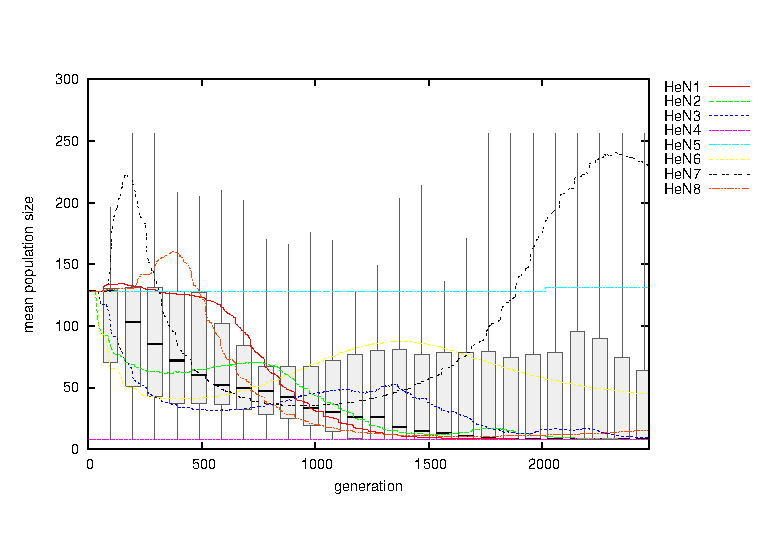
\includegraphics[width =8.0cm] {mmdp-size-300-mut-0.003-xover-1-heterohardware-adaptsize.eps}
   \label{subfig:adaptMMDP300}
}

\subfigure[15000 OneMax]{
    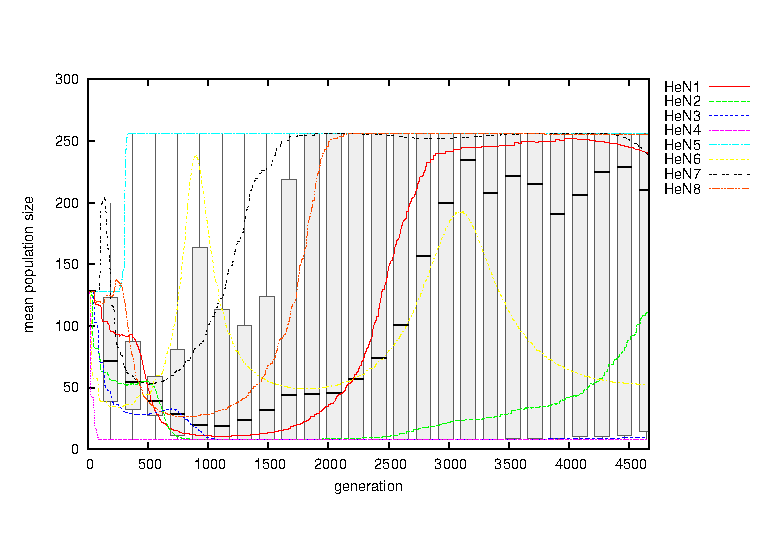
\includegraphics[width =8.0cm] {onemax-size-15000-mut-0.00006-xover-1-heterohardware-adaptsize.eps}
    \label{subfig:adaptONEMAX15000}
}

\subfigure[50 Rosenbrock]{
    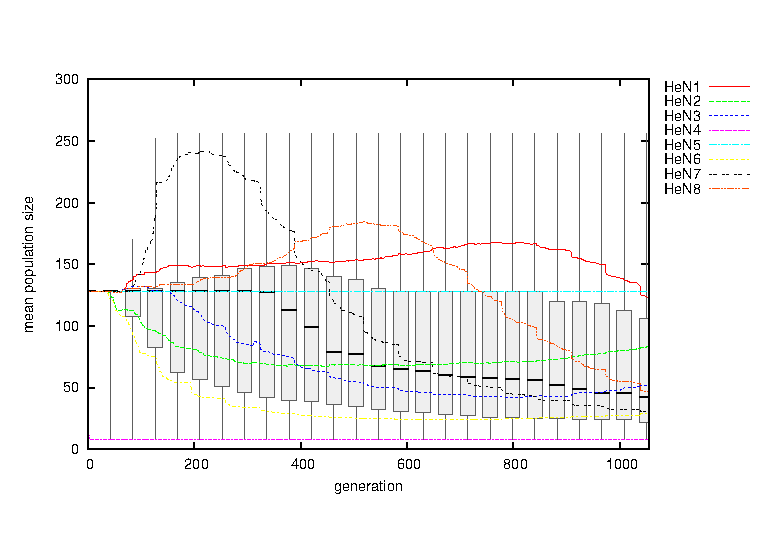
\includegraphics[width =8.0cm] {cec-size-50-mut-0.02-xover-1-heterohardware-adaptsize.eps}
    \label{subfig:adaptROSENBROCK50}
}
\caption{Average sizes of all the sub-populations during all the runs (boxplots), and the average size of each node sub-population (lines), for the 8X/AdSi.}
\label{fig:adaptivesize}
\end{figure}




\subsection{Running time of each stage of the algorithm}

As a final analysis the time spent by each node of the clusters on
every stage of the EA for each configuration with fixed sizes (HoSi
and HeSi) is taken into account. For the sake of clarity in results, 
 the 4X configuration for the smallest instance of each problem is shown. Figure \ref{fig:bars} compares these results. As can be seen, the migration is the most time consuming operation in all configurations, being the migration in HeHW more expensive than in HoHW. This happens because a multi-purpose laboratory network to communicate
the nodes is being used, instead of the specific one used in the HoHW
system. 

 In problems with larger data communications (300 or 5000 elements of individuals of the MMDP and OneMax problem) changing the sub-population size decreases the migration time in HeHW, but increases in HoHW. This might be due to the synchronization of migration buffers: if all machines are sending/receiving at the same time, bottlenecks can be propagated.

\begin{figure}[ht]
\centering
\subfigure{
   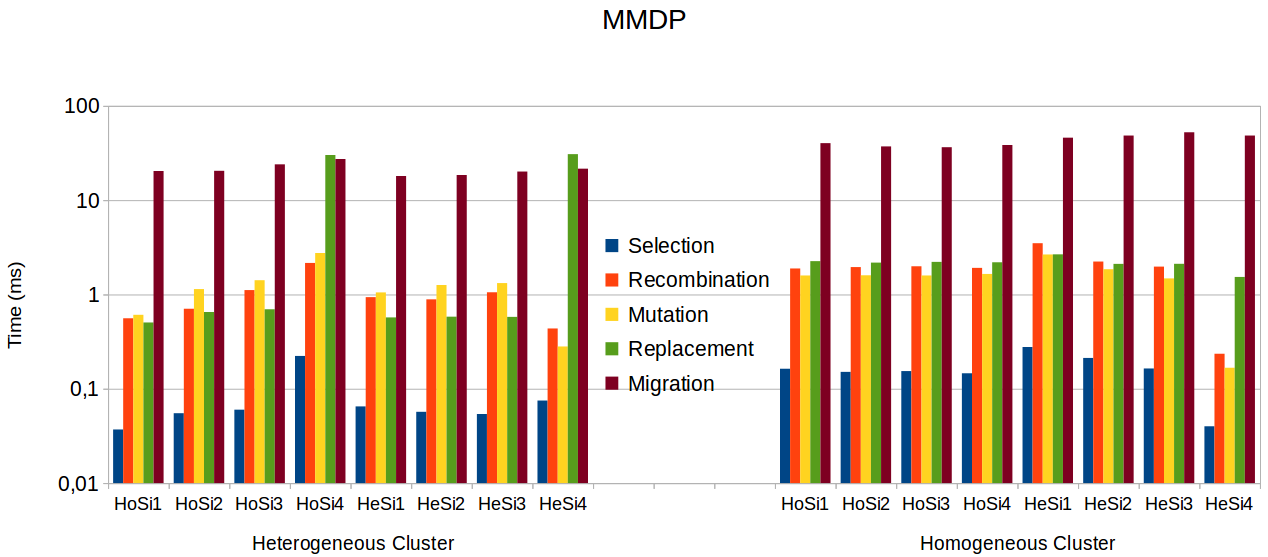
\includegraphics[scale =0.3] {mmdpbars.eps}
   \label{subfig:mmdpbars}
 }
\subfigure{
   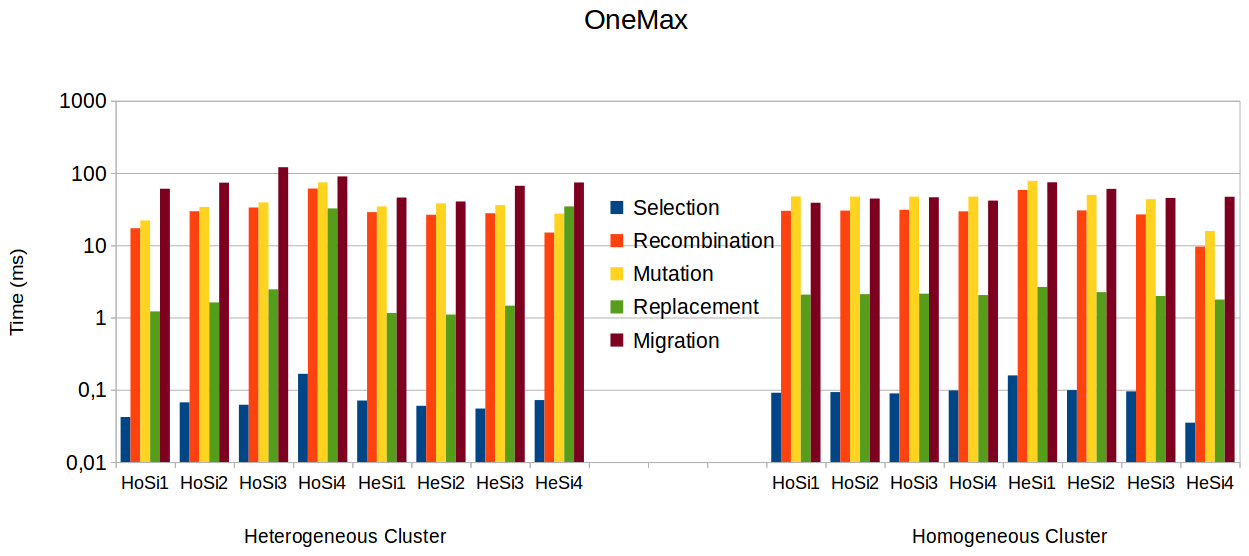
\includegraphics[scale =0.3] {onemaxbars.eps}
   \label{subfig:onemaxbars}
 }
 \subfigure{
   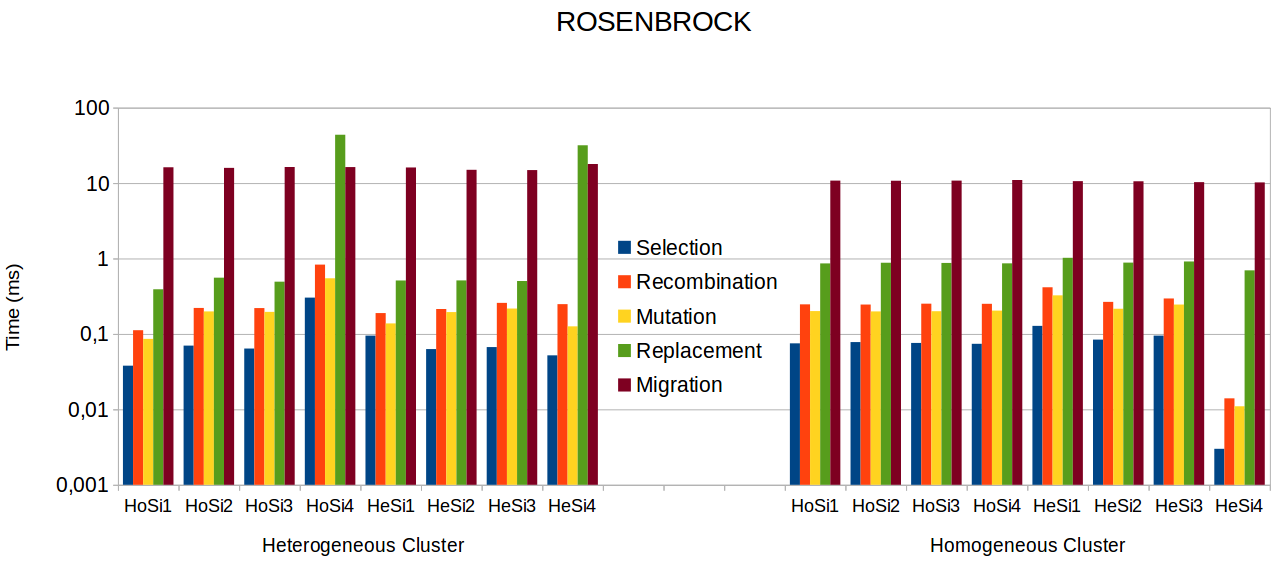
\includegraphics[scale =0.3] {rosenbrockbars.eps}
   \label{subfig:rosenbrockbars}
 }
\caption{Average time spent on each section of the algorithm for each node (milliseconds).}
\label{fig:bars}
\end{figure}



Results also show how the stages of the algorithms depend on the execution
node. For example, the node HeN4 requires a lot of time in the replacement stage,
 as it is the only one that writes into the log files. This node was the only one
  using network storage (see Table \ref{tabcomputers}).

Different proportion of time can be spent on each section depending on the problem.
The reason might be the
creation of new objects (memory allocation), which in Java and with
limited memory (and swapping) requires more time than the iteration of
elements previously created, for example, in the mutation. Fitting
the sub-population size makes the slowest node of HeHW behave in similar
way than the other nodes (same time on each stage). Moreover, the size
of the individuals affects some parts of the EA; for example, in 
OneMax the mutation requires higher time than the replacement. However,
it must be taken into account that the time spent in each part of the
algorithm is not related to the time needed to reach the optimum, but to
how the diversity and search guidance is maintained in the whole
system.  



\section{Conclusions and future work}



The main question addressed in this work was: Is it worth fitting the 
sub-populations sizes of a dEA to the computational power of each node 
in a heterogeneous cluster? To answer this question properly a set of 
experiments was designed with several characteristics in mind. 
First, the separate study of two parameter settings: offline and 
online. Also, the usage of three problems with different characteristics and 
computational demands with different lengths. Finally, two different hardware 
systems (homogeneous and heterogeneous clusters),  each one with different number
 of nodes (4 and 8).

A base configuration with the same sub-population sizes was used on a heterogeneous cluster. The results were used to calculate offline the computational power of each node, comparing the average number of generations to find the optimal solution. These proportions were used to set the new sub-population sizes. Also, a possible way to fit online the sub-population sizes was performed comparing the current generation number between each node and its previous neighbour in the topology. 

Results showed that online or offline fitting the sub-population size to the computational power of each node in a heterogeneous cluster
can reduce significantly the running time of an algorithm with respect
to keeping the same size for all nodes. The sub-population size fitting was also affected by the problem being solved. Also, to answer the question about the difference of using these same sub-populations sizes in a homogeneous cluster, a control system was also used for comparison. In this case, the same parameter sets used in a homogeneous cluster did not improve the running time in multi-modal problems, as the average fitness of the population remained close to the average best fitness during all the evolution, and therefore, fitness diversity was not as well maintained as in the heterogeneous cluster.



Furthermore, the answer to the question about the influence of the sub-population size effect on the stages
of the algorithm was that, in fact, there existed an effect on stages that are independent of this parameter, such as
the migration.  These results are a promising start for fitting EAs to the performance of each  node, using more suitable benchmarks or even in a dynamic way. 

In a future work, new online adaptation methods for sub-population sizes will take into account the nature of the problem at hand. For example, measuring the population diversity along with the generation number. Also, parameters such as migration rate or crossover probability could be fitted to the node's execution characteristics. Other appropriate benchmarks to analyse the algorithm will be used to get an online automatic parameter fitting while nodes enter or exit the topology net, or fitting the parameters to the current system load.

\section*{Acknowledgements}
This work has been supported in part by SIPESCA (Programa Operativo FEDER de Andaluc{\'i}a 2007-2013), TIN2011-28627-C04-02 and TIN2014-56494-C4-3-P (Spanish Ministry of Economy and Competitivity), SPIP2014-01437 (Direcci{\'o}n General de Tr{\'a}fico), PRY142/14 (Fundaci{\'o}n P{\'u}blica Andaluza, Centro de Estudios Andaluces en la IX Convocatoria de Proyectos de Investigaci{\'o}n), and PYR-2014-17 GENIL project (CEI-BIOTIC Granada). Authors wish to thank the reviewers' comments, whose suggestion and guidelines have contributed to improve this work.



%% The Appendices part is started with the command \appendix;
%% appendix sections are then done as normal sections
%% \appendix

%% \section{}
%% \label{}

%% References
%%
%% Following citation commands can be used in the body text:
%% Usage of \cite is as follows:
%%   \cite{key}         ==>>  [#]
%%   \cite[chap. 2]{key} ==>> [#, chap. 2]
%%

%% References with bibTeX database:

%\bibliographystyle{elsarticle-num}
%\bibliography{AMIVITAL-ESA}

%% Authors are advised to submit their bibtex database files. They are
%% requested to list a bibtex style file in the manuscript if they do
%% not want to use elsarticle-num.bst.

%% References without bibTeX database:

% \begin{thebibliography}{00}

%% \bibitem must have the following form:
%%   \bibitem{key}...
%%

% \bibitem{}

% \end{thebibliography}




%\bibliographystyle{plain}
%\bibliography{heterogeneous}
%Descomentar abajo cuando comentes arriba
%\section*{References}



\begin{thebibliography}{10}

\bibitem{Acosta13GPUs}
Alejandro Acosta, Vicente Blanco, and Francisco Almeida.
\newblock Dynamic load balancing on heterogeneous multi-gpu systems.
\newblock {\em Computers \& Electrical Engineering}, 39(8):2591 -- 2602, 2013.

\bibitem{EVALUATIONPARALLEL}
Enrique Alba and Gabriel Luque.
\newblock Evaluation of parallel metaheuristics.
\newblock In Lu\'is Paquete, Marco Chiarandini, and Dario Basso, editors, {\em
  Empirical Methods for the Analysis of Algorithms, Workshop EMAA 2006,
  Proceedings}, pages 9--14, Reykjavik, Iceland, 2006.

\bibitem{HETEROGENEOUSHARD}
Enrique Alba, Antonio~J. Nebro, and Jos\'e~M. Troya.
\newblock Heterogeneous computing and parallel genetic algorithms.
\newblock {\em Journal of Parallel and Distributed Computing}, 62(9):1362 --
  1385, 2002.

\bibitem{alba2002parallelism}
Enrique Alba and Marco Tomassini.
\newblock Parallelism and evolutionary algorithms.
\newblock {\em Evolutionary Computation, IEEE Transactions on}, 6(5):443--462,
  2002.

\bibitem{OPENSCIENCEGRID}
Mine Altunay, Paul Avery, Kent Blackburn, Brian Bockelman, Michael Ernst, Dan
  Fraser, Robert Quick, Robert Gardner, Sebastien Goasguen, Tanya Levshina,
  Miron Livny, John McGee, Doug Olson, Ruth Pordes, Maxim Potekhin, Abhishek
  Rana, Alain Roy, Chander Sehgal, Igor Sfiligoi, Frank Wuerthwein, and {Open
  Sci Grid Executive Board}.
\newblock {A Science Driven Production Cyberinfrastructure-the Open Science
  Grid}.
\newblock {\em {Journal of GRID Computing}}, {9}({2, Sp. Iss. SI}):{201--218},
  {JUN} 2011.

\bibitem{MULTIKULTI}
Lourdes Araujo and Juan J.~Merelo Guerv{\'o}s.
\newblock Diversity through multiculturality: Assessing migrant choice policies
  in an island model.
\newblock {\em IEEE Trans. Evolutionary Computation}, 15(4):456--469, 2011.

\bibitem{LoadBalancingBohn02}
Christopher~A. Bohn and Gary~B. Lamont.
\newblock Load balancing for heterogeneous clusters of {PCs}.
\newblock {\em Future Generation Computer Systems}, 18(3):389 -- 400, 2002.

\bibitem{CantuPazTopologies99}
Erick Cant{\'{u}}{-}Paz.
\newblock Topologies, migration rates, and multi-population parallel genetic
  algorithms.
\newblock In Wolfgang Banzhaf, Jason~M. Daida, Agoston~E. Eiben, Max~H. Garzon,
  Vasant Honavar, Mark~J. Jakiela, and Robert~E. Smith, editors, {\em
  Proceedings of the Genetic and Evolutionary Computation Conference {(GECCO}
  1999), 13-17 July 1999, Orlando, Florida, {USA}}, pages 91--98. Morgan
  Kaufmann, 1999.

\bibitem{Cantu02Multiple}
Erick Cant{\'{u}}{-}Paz and David~E. Goldberg.
\newblock Are multiple runs of genetic algorithms better than one?
\newblock In Erick Cant{\'{u}}{-}Paz, James~A. Foster, Kalyanmoy Deb, Lawrence
  Davis, Rajkumar Roy, Una{-}May O'Reilly, Hans{-}Georg Beyer, Russell~K.
  Standish, Graham Kendall, Stewart~W. Wilson, Mark Harman, Joachim Wegener,
  Dipankar Dasgupta, Mitchell~A. Potter, Alan~C. Schultz, Kathryn~A. Dowsland,
  Natasa Jonoska, and Julian~F. Miller, editors, {\em Genetic and Evolutionary
  Computation - {GECCO} 2003, Genetic and Evolutionary Computation Conference,
  Chicago, IL, USA, July 12-16, 2003. Proceedings, Part {I}}, volume 2723 of
  {\em Lecture Notes in Computer Science}, pages 801--812. Springer, 2003.

\bibitem{PanaceasClune05}
Jeff Clune, Sherri Goings, Bill Punch, and Eric Goodman.
\newblock Investigations in meta-{GAs}: panaceas or pipe dreams?
\newblock In Franz Rothlauf, editor, {\em Genetic and Evolutionary Computation
  Conference, {GECCO} 2005, Workshop Proceedings, Washington DC, USA, June
  25-26, 2005}, pages 235--241. {ACM}, 2005.

\bibitem{Derby13Cloud}
Owen Derby, Kalyan Veeramachaneni, and Una{-}May O'Reilly.
\newblock Cloud driven design of a distributed genetic programming platform.
\newblock In Anna~Isabel Esparcia{-}Alc{\'{a}}zar, editor, {\em Applications of
  Evolutionary Computation - 16th European Conference, EvoApplications 2013,
  Vienna, Austria, April 3-5, 2013. Proceedings}, volume 7835 of {\em Lecture
  Notes in Computer Science}, pages 509--518. Springer, 2013.

\bibitem{Dominguez13HydroCM}
Juli{\'{a}}n Dom{\'{\i}}nguez and Enrique Alba.
\newblock Dealing with hardware heterogeneity: a new parallel search model.
\newblock {\em Natural Computing}, 12(2):179--193, 2013.

\bibitem{HYDROCM}
Juli{\'{a}}n Dom{\'{\i}}nguez and Enrique Alba.
\newblock Hydrocm: {A} hybrid parallel search model for heterogeneous
  platforms.
\newblock In El{-}Ghazali Talbi, editor, {\em Hybrid Metaheuristics}, volume
  434 of {\em Studies in Computational Intelligence}, pages 219--235. Springer,
  2013.

\bibitem{LinpackDongarra03}
Jack~J. Dongarra, Piotr Luszczek, and Antoine Petitet.
\newblock The {LINPACK} benchmark: Past, present, and future.
\newblock {\em Concurrency and Computation: Practice and Experience}, 15:2003,
  2003.

\bibitem{Eiben05Shared}
Agoston~E. Eiben.
\newblock Evolutionary computing and autonomic computing: Shared problems,
  shared solutions?
\newblock In {\"{O}}zalp Babaoglu, M{\'{a}}rk Jelasity, Alberto Montresor,
  Christof Fetzer, Stefano Leonardi, Aad P.~A. van Moorsel, and Maarten van
  Steen, editors, {\em Self-star Properties in Complex Information Systems,
  Conceptual and Practical Foundations [the book is a result from a workshop at
  Bertinoro, Italy, Summer 2004]}, volume 3460 of {\em Lecture Notes in
  Computer Science}, pages 36--48. Springer, 2005.

\bibitem{PARAMETERTUNING}
Agoston~E. Eiben and Selmar~K. Smit.
\newblock Parameter tuning for configuring and analyzing evolutionary
  algorithms.
\newblock {\em Swarm and Evolutionary Computation}, 1(1):19--31, 2011.

\bibitem{GeneticAlgorithmsEiben03}
Agoston~E. Eiben and James~E. Smith.
\newblock Genetic algorithms.
\newblock In {\em Introduction to Evolutionary Computing}, Natural Computing
  Series, pages 37--70. Springer Berlin Heidelberg, 2003.

\bibitem{LinpackEndo10}
Toshio Endo, Akira Nukada, Satoshi Matsuoka, and Naoya Maruyama.
\newblock Linpack evaluation on a supercomputer with heterogeneous
  accelerators.
\newblock In {\em 24th {IEEE} International Symposium on Parallel and
  Distributed Processing, {IPDPS} 2010, Atlanta, Georgia, USA, 19-23 April 2010
  - Conference Proceedings}, pages 1--8. {IEEE}, 2010.

\bibitem{SelfRegulatedSizeFernandes06}
Carlos~M. Fernandes and Agostinho~C. Rosa.
\newblock Self-regulated population size in evolutionary algorithms.
\newblock In Thomas~Philip Runarsson, Hans{-}Georg Beyer, Edmund~K. Burke, Juan
  J.~Merelo Guerv{\'{o}}s, L.~Darrell Whitley, and Xin Yao, editors, {\em
  Parallel Problem Solving from Nature - {PPSN} IX, 9th International
  Conference, Reykjavik, Iceland, September 9-13, 2006, Procedings}, volume
  4193 of {\em Lecture Notes in Computer Science}, pages 920--929. Springer,
  2006.

\bibitem{GLOBUS}
Ian~T. Foster.
\newblock Globus toolkit version 4: Software for service-oriented systems.
\newblock {\em J. Comput. Sci. Technol.}, 21(4):513--520, 2006.

\bibitem{PARALLELIMPLEMENTATION}
Juan~Francisco Garamendi and Jos{\'{e}}~L. Bosque.
\newblock Parallel implementation of evolutionary strategies on heterogeneous
  clusters with load balancing.
\newblock In {\em 20th International Parallel and Distributed Processing
  Symposium {(IPDPS} 2006), Proceedings, 25-29 April 2006, Rhodes Island,
  Greece}. {IEEE}, 2006.

\bibitem{SOASOCO}
Pablo Garc{\'{\i}}a{-}S{\'{a}}nchez, Jes{\'{u}}s~Gonz{\'{a}}lez, Pedro~A. Castillo,
  Maribel~Garc{\'{\i}}a Arenas, and Juan J.~Merelo Guerv{\'{o}}s.
\newblock Service oriented evolutionary algorithms.
\newblock {\em Soft Comput.}, 17(6):1059--1075, 2013.

\bibitem{goldberg92massive}
David~E. Goldberg, Kalyanmoy Deb, and Jeffrey Horn.
\newblock Massive multimodality, deception, and genetic algorithms.
\newblock In Reinhard M{\"{a}}nner and Bernard Manderick, editors, {\em
  Parallel Problem Solving from Nature 2, PPSN-II, Brussels, Belgium, September
  28-30, 1992}, pages 37--48. Elsevier, 1992.

\bibitem{HETEROGENEOUSPARAMETERS}
Yiyuan Gong and Alex Fukunaga.
\newblock Distributed island-model genetic algorithms using heterogeneous
  parameter settings.
\newblock In {\em Proceedings of the {IEEE} Congress on Evolutionary
  Computation, {CEC} 2011, New Orleans, LA, USA, 5-8 June, 2011}, pages
  820--827. {IEEE}.

\bibitem{HETEROGENEOUSTOPOLOGY}
Yiyuan Gong, Morikazu Nakamura, and Shiro Tamaki.
\newblock Parallel genetic algorithms on line topology of heterogeneous
  computing resources.
\newblock In Hans{-}Georg Beyer and Una{-}May O'Reilly, editors, {\em Genetic
  and Evolutionary Computation Conference, {GECCO} 2005, Proceedings,
  Washington DC, USA, June 25-29, 2005}, pages 1447--1454. {ACM}, 2005.

\bibitem{AsynchronousMerelo08}
Juan J.~Merelo Guerv{\'{o}}s, Pedro A.~Castillo Valdivieso, Juan
  L.~Jim{\'{e}}nez Laredo, Antonio~Mora Garc{\'{\i}}a, and Alberto
  Prieto.
\newblock Asynchronous distributed genetic algorithms with javascript and
  {JSON}.
\newblock In {\em Proceedings of the {IEEE} Congress on Evolutionary
  Computation, {CEC} 2008, June 1-6, 2008, Hong Kong, China}, pages 1372--1379.
  {IEEE}, 2008.

\bibitem{SizingHarik99}
George Harik, Erick Cant\'{u}-Paz, David~E. Goldberg, and Brad~L. Miller.
\newblock The gambler's ruin problem, genetic algorithms, and the sizing of
  populations.
\newblock {\em Evolutionary Computation}, 7(3):231--253, September 1999.

\bibitem{ShrinkageLaredo09}
Juan L.~Jim{\'{e}}nez Laredo, Carlos~M. Fernandes, Juan
  J.~Merelo Guerv{\'{o}}s, and Christian Gagn{\'{e}}.
\newblock Improving genetic algorithms performance via deterministic population
  shrinkage.
\newblock In Franz Rothlauf, editor, {\em Genetic and Evolutionary Computation
  Conference, {GECCO} 2009, Proceedings, Montreal, Qu{\'{e}}bec, Canada, July
  8-12, 2009}, pages 819--826. {ACM}, 2009.

\bibitem{AdaptiveLobo07}
Fernando~G. Lobo and Cl\'{a}udio~F. Lima.
\newblock Adaptive population sizing schemes in genetic algorithms.
\newblock In Fernando~G. Lobo, Cl\'{a}udio~F. Lima, and Zbigniew Michalewicz,
  editors, {\em Parameter Setting in Evolutionary Algorithms}, volume~54 of
  {\em Studies in Computational Intelligence}, pages 185--204. Springer Berlin
  Heidelberg, 2007.

\bibitem{Martinez11Nondedicated}
Jose~A. Mart{\'{\i}}nez, Francisco Almeida, Ester~M. Garz{\'{o}}n, Alejandro
  Acosta, and Vicente~Blanco P{\'{e}}rez.
\newblock Adaptive load balancing of iterative computation on heterogeneous
  nondedicated systems.
\newblock {\em The Journal of Supercomputing}, 58(3):385--393, 2011.

\bibitem{Robles09ParallelFuzzy}
Ignacio Robles, Rafael Alcal{\'{a}}, Jos{\'{e}}~Manuel Ben{\'{\i}}tez, and
  Francisco Herrera.
\newblock Evolutionary parallel and gradually distributed lateral tuning of
  fuzzy rule-based systems.
\newblock {\em Evolutionary Intelligence}, 2(1-2):5--19, 2009.

\bibitem{HETEROGENEOUSMIGRATION}
Carolina Salto and Enrique Alba.
\newblock Designing heterogeneous distributed gas by efficiently self-adapting
  the migration period.
\newblock {\em Applied Intelligence}, 36:800--808, 2012.

\bibitem{Salto13Distributed}
Carolina Salto, Francisco Luna, and Enrique Alba.
\newblock Distributed evolutionary algorithms in heterogeneous environments.
\newblock In Fatos Xhafa, Leonard Barolli, Dritan Nace, Salvatore Venticinque,
  and Alain Bui, editors, {\em Eighth International Conference on P2P,
  Parallel, Grid, Cloud and Internet Computing, 3PGCIC 2013, Compiegne, France,
  October 28-30, 2013}, pages 606--611. {IEEE}, 2013.

\bibitem{ONEMAX}
J.~David Schaffer and Larry~J. Eshelman.
\newblock On crossover as an evolutionarily viable strategy.
\newblock In Richard~K. Belew and Lashon~B. Booker, editors, {\em Proceedings
  of the 4th International Conference on Genetic Algorithms, San Diego, CA,
  USA, July 1991}, pages 61--68. Morgan Kaufmann, 1991.

\bibitem{AdaptationSizesSchlierkamp96}
Dirk Schlierkamp{-}Voosen and Heinz M{\"{u}}hlenbein.
\newblock Adaptation of population sizes by competing subpopulations.
\newblock In {\em International Conference on Evolutionary Computation}, pages
  330--335, 1996.

\bibitem{AutomaticallyConfiguringStyles12}
James Styles, Holger H. Hoos, and Martin M{\"{u}}ller.
\newblock Automatically configuring algorithms for scaling performance.
\newblock In Youssef Hamadi and Marc Schoenauer, editors, {\em Learning and
  Intelligent Optimization}, Lecture Notes in Computer Science, pages 205--219.
  Springer Berlin Heidelberg, 2012.

\bibitem{CEC2005_Benchmark}
Ponnuthurai~N. Suganthan, Nikolaus~Hansen, Jing~J. Liang, Kalyanmoy~Deb, Ying~P. Chen, Anne~Auger, and
  Santosh~Tiwari.
\newblock Problem definitions and evaluation criteria for the cec 2005 special
  session on real-parameter optimization.
\newblock Technical report, Nanyang Technological University, Singapore, 2005.
\newblock http://www.ntu.edu.sg/home/EPNSugan.

\bibitem{tanabe2013evaluation}
Ryoji Tanabe and Alex Fukunaga.
\newblock Evaluation of a randomized parameter setting strategy for
  island-model evolutionary algorithms.
\newblock In {\em Proceedings of the {IEEE} Congress on Evolutionary
  Computation, {CEC} 2013, Cancun, Mexico, June 20-23, 2013}, pages 1263--1270.
  {IEEE}, 2013.

\bibitem{ParallelGATongchim02}
Shisanu Tongchim and Prabhas Chongstitvatana.
\newblock Parallel genetic algorithm with parameter adaptation.
\newblock {\em Inf. Process. Lett.}, 82(1):47--54, 2002.

\bibitem{garcia2014randomized}
Mario~Garc{\'{\i}}a Valdez, Leonardo Trujillo, Juan J.~Merelo
  Guerv{\'{o}}s, and Francisco~Fern{\'{a}}ndez de~Vega.
\newblock Randomized parameter settings for heterogeneous workers in a
  pool-based evolutionary algorithm.
\newblock In Thomas Bartz{-}Beielstein, J{\"{u}}rgen Branke, Bogdan Filipic,
  and Jim Smith, editors, {\em Parallel Problem Solving from Nature - {PPSN}
  {XIII} - 13th International Conference, Ljubljana, Slovenia, September 13-17,
  2014. Proceedings}, volume 8672 of {\em Lecture Notes in Computer Science},
  pages 702--710. Springer, 2014.

\bibitem{Verma09MapReduce}
Abhishek Verma, Xavier Llor{\`{a}}, David~E. Goldberg, and Roy~H. Campbell.
\newblock Scaling genetic algorithms using mapreduce.
\newblock In {\em Ninth International Conference on Intelligent Systems Design
  and Applications, {ISDA} 2009, Pisa, Italy , November 30-December 2, 2009},
  pages 13--18. {IEEE} Computer Society, 2009.

\bibitem{Wakunda97EVA}
J{\"{u}}rgen Wakunda and Andreas Zell.
\newblock Eva - {A} tool for optimization with evolutionary algorithms.
\newblock In {\em 23rd {EUROMICRO} Conference '97, New Frontiers of Information
  Technology, 1-4 September 1997, Budapest, Hungary}, page 644. {IEEE} Computer
  Society, 1997.

\bibitem{DifferentialWeber09}
Matthieu Weber, Ferrante Neri, and Ville Tirronen.
\newblock Distributed differential evolution with explorative-exploitative
  population families.
\newblock {\em Genetic Programming and Evolvable Machines}, 10(4):343--371,
  2009.

\bibitem{Wolpert97NFL}
David Wolpert and William~G. Macready.
\newblock No free lunch theorems for optimization.
\newblock {\em {IEEE} Trans. Evolutionary Computation}, 1(1):67--82, 1997.



\end{thebibliography}

\end{document}

%%
%% End of file `elsarticle-template-num.tex'.
